\documentclass[11pt]{article}
\usepackage{amsmath}
\usepackage{graphicx}
\usepackage{subcaption}
\usepackage{booktabs}
\usepackage{float}
\usepackage[margin=1in]{geometry}

\title{CS5330 --- Project 5: Recognition using Deep Networks}
\author{Ashish Dasu}
\date{April 2026}

\begin{document}
\maketitle

% ---------------------------------------------------------------
\section{Project Overview}
% ---------------------------------------------------------------

This project explores deep learning for image recognition through six
tasks. A convolutional neural network (CNN) is trained on MNIST
handwritten digits, examined at the filter level, and extended via
transfer learning to classify Greek letters. A vision transformer is
re-implemented and compared to the CNN. A systematic experiment on
Fashion MNIST evaluates how three architectural dimensions affect
performance. Six extensions are presented: live webcam digit
recognition, additional Greek letter classes with domain shift
analysis, a Gabor filter bank comparison, confusion matrix analysis,
t-SNE embedding visualization, and a data augmentation experiment.

% ---------------------------------------------------------------
\section{Task 1 --- Build and Train CNN on MNIST}
% ---------------------------------------------------------------

\subsection{Network Architecture}

The CNN takes a single-channel 28$\times$28 grayscale image and
produces log-probabilities over 10 digit classes. The architecture
follows the assignment specification exactly.

\begin{figure}[H]
    \centering
    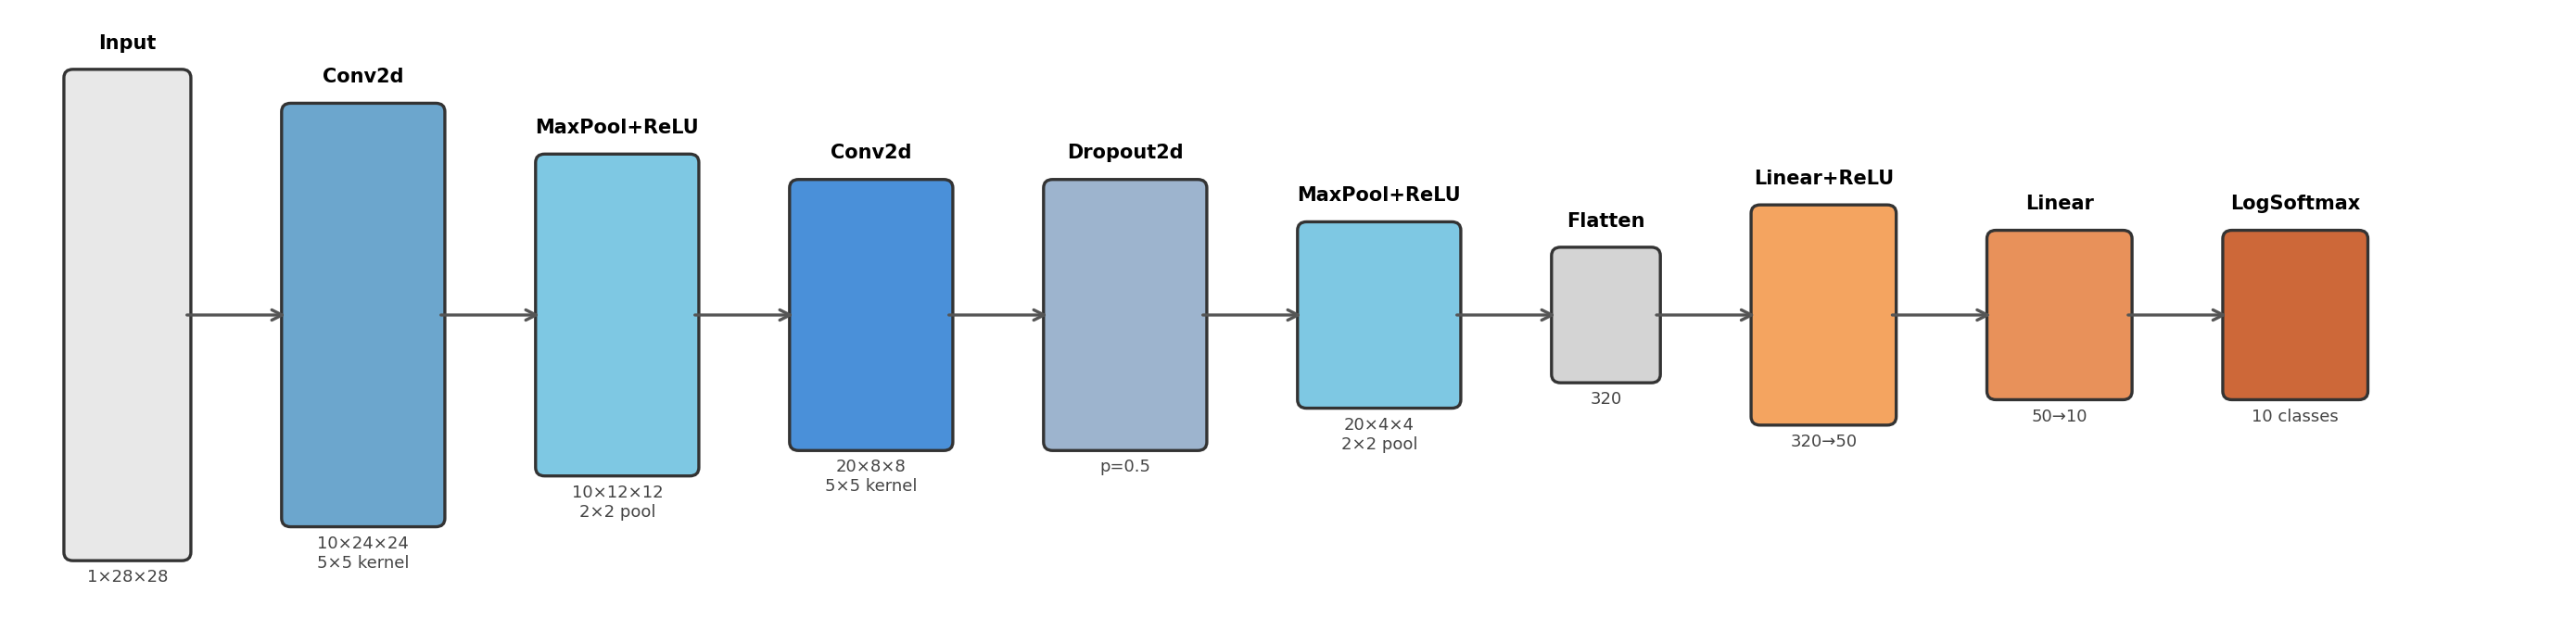
\includegraphics[width=\textwidth]{report_images/cnn_architecture.png}
    \caption{CNN architecture. Two convolutional layers extract spatial
    features, each followed by 2$\times$2 max pooling and ReLU. Dropout
    (p=0.5) regularizes after the second convolution. Two fully connected
    layers map the 320-dimensional flattened features to 10 class
    probabilities via log-softmax.}
\end{figure}

\subsection{Training}

The network was trained for 5 epochs on MNIST (60k training, 10k test)
using SGD (lr=0.01, momentum=0.5) with batch size 64 and negative
log-likelihood loss. MPS acceleration was used on an Apple M1 MacBook
Pro. The trained model was saved to \texttt{mnist\_model.pth} for
reuse in subsequent tasks.

\subsection{First 6 Test Examples}

\begin{figure}[H]
    \centering
    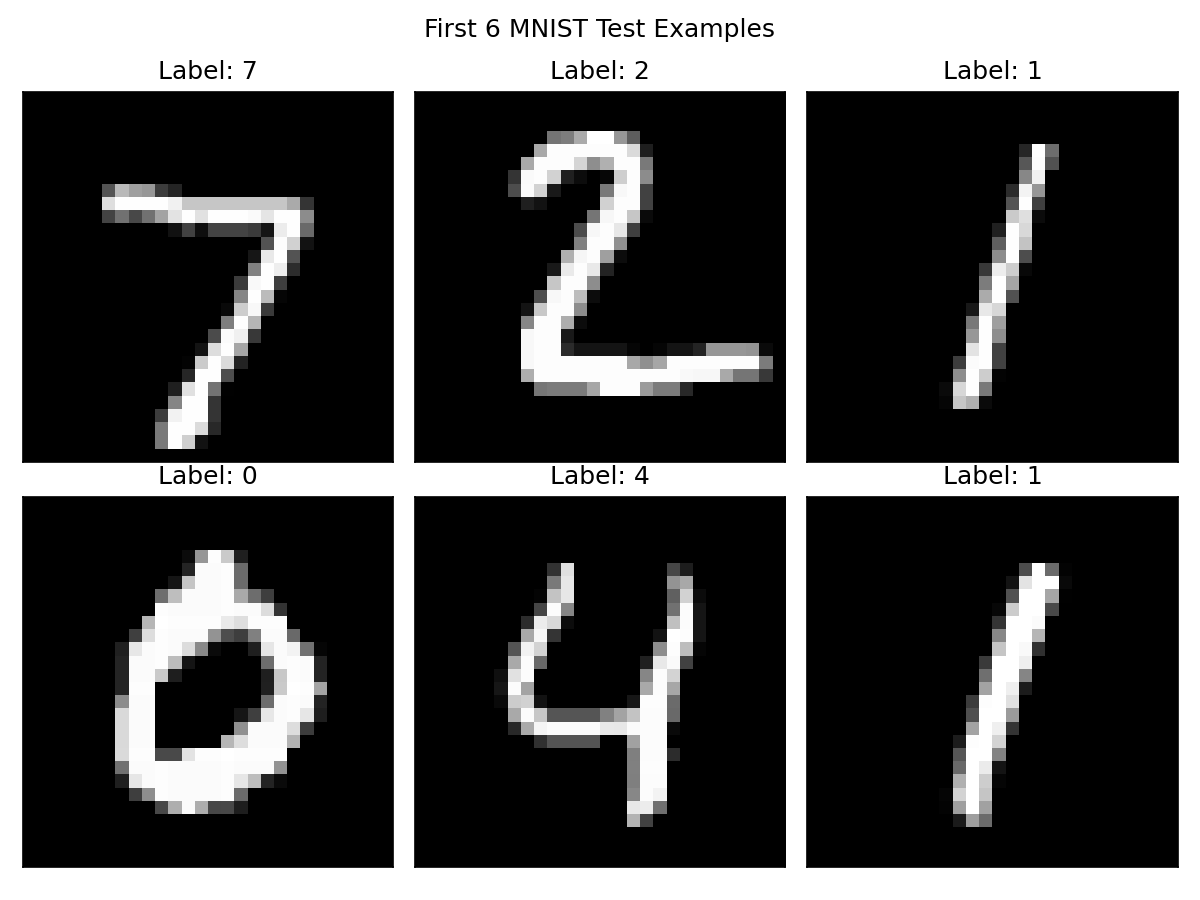
\includegraphics[width=0.6\textwidth]{report_images/first_six_test.png}
    \caption{First 6 images from the MNIST test set displayed in a
    2$\times$3 grid with their ground-truth labels.}
\end{figure}

\subsection{Training Results}

\begin{figure}[H]
    \centering
    \begin{subfigure}[b]{0.48\textwidth}
        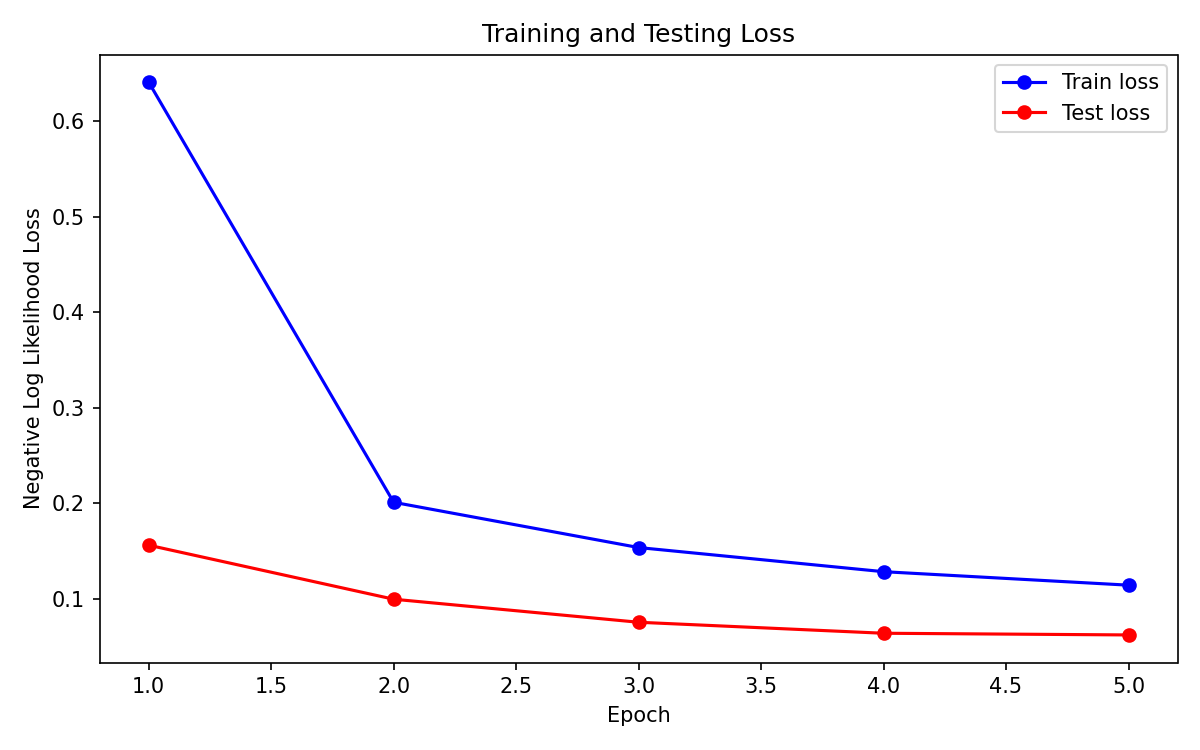
\includegraphics[width=\textwidth]{report_images/loss_plot.png}
        \caption{Loss}
    \end{subfigure}
    \hfill
    \begin{subfigure}[b]{0.48\textwidth}
        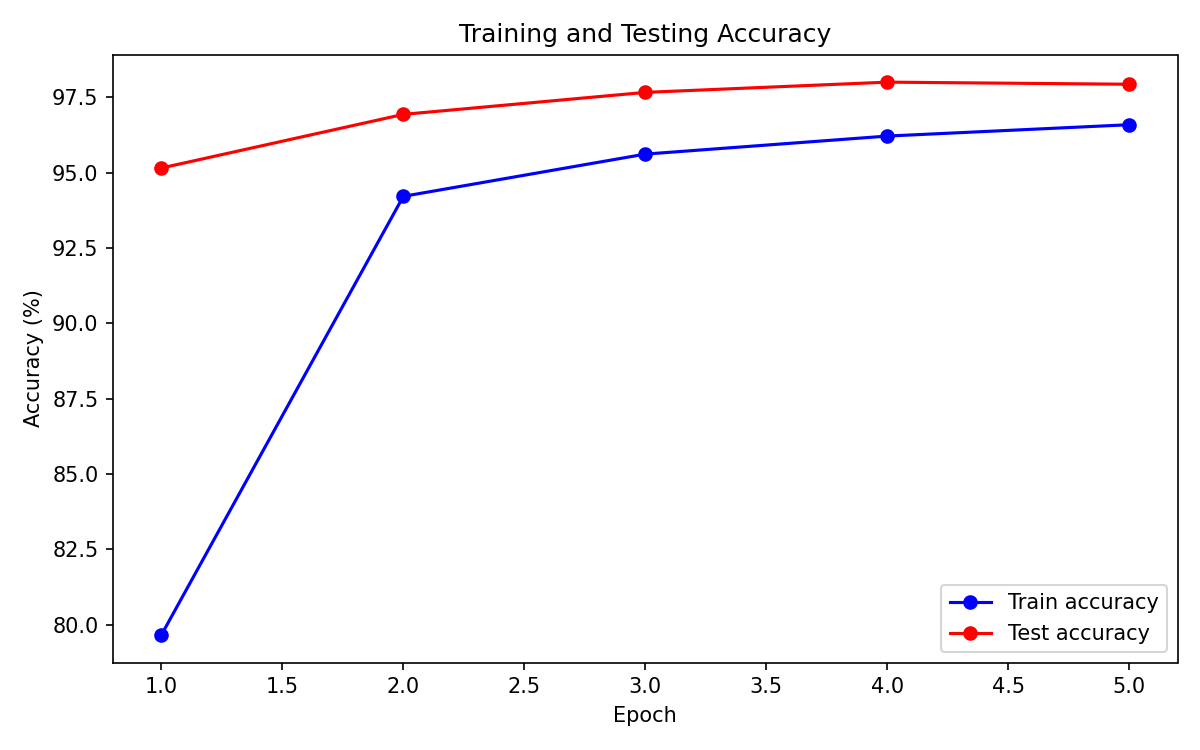
\includegraphics[width=\textwidth]{report_images/accuracy_plot.png}
        \caption{Accuracy}
    \end{subfigure}
    \caption{Training and testing curves across 5 epochs. Test accuracy
    reaches 97.93\% with the gap between training and testing loss
    remaining small, indicating effective generalization.}
\end{figure}

\begin{table}[H]
    \centering
    \begin{tabular}{ccccc}
        \toprule
        Epoch & Train Loss & Test Loss & Train Acc & Test Acc \\
        \midrule
        1 & 0.6409 & 0.1560 & 79.66\% & 95.15\% \\
        2 & 0.2009 & 0.0994 & 94.21\% & 96.93\% \\
        3 & 0.1535 & 0.0752 & 95.61\% & 97.66\% \\
        4 & 0.1282 & 0.0637 & 96.21\% & 98.00\% \\
        5 & 0.1141 & 0.0620 & 96.59\% & 97.93\% \\
        \bottomrule
    \end{tabular}
    \caption{Per-epoch training metrics. The network converges rapidly,
    with most improvement in the first two epochs.}
\end{table}

% ---------------------------------------------------------------
\section{Task 2 --- Evaluate on Test Set and Handwritten Digits}
% ---------------------------------------------------------------

\subsection{Test Set Evaluation}

The saved model was loaded and set to evaluation mode via
\texttt{model.eval()}, which disables dropout so all neurons
contribute to predictions during inference. The first 10 test examples
were then run through the network. For each example, all 10
log-probability output values were recorded along with the predicted
and true labels. The network correctly classifies all 10 examples with
high confidence.

\begin{table}[H]
    \centering
    \footnotesize
    \begin{tabular}{ccccccccccccc}
        \toprule
        Idx & 0 & 1 & 2 & 3 & 4 & 5 & 6 & 7 & 8 & 9 & Pred & True \\
        \midrule
        0 & -19.02 & -17.31 & -12.71 & -11.46 & -21.04 & -19.76 & -34.03 & \textbf{-0.00} & -16.96 & -12.51 & 7 & 7 \\
        1 & -7.78 & -7.66 & \textbf{-0.00} & -14.41 & -18.39 & -19.81 & -9.08 & -19.56 & -10.00 & -23.47 & 2 & 2 \\
        2 & -13.16 & \textbf{-0.00} & -10.24 & -14.41 & -8.95 & -13.27 & -12.66 & -8.85 & -12.13 & -13.88 & 1 & 1 \\
        3 & \textbf{-0.00} & -23.64 & -13.41 & -19.58 & -18.21 & -14.82 & -12.13 & -13.14 & -15.87 & -12.84 & 0 & 0 \\
        4 & -18.68 & -19.90 & -14.38 & -15.78 & \textbf{-0.00} & -14.27 & -16.31 & -12.96 & -14.73 & -7.40 & 4 & 4 \\
        5 & -15.70 & \textbf{-0.00} & -12.71 & -16.64 & -10.23 & -16.64 & -16.75 & -9.43 & -14.48 & -15.65 & 1 & 1 \\
        6 & -23.43 & -12.05 & -14.66 & -12.50 & \textbf{-0.00} & -12.55 & -22.81 & -7.25 & -8.27 & -6.37 & 4 & 4 \\
        7 & -18.33 & -14.39 & -11.45 & -8.10 & -6.69 & -11.19 & -22.58 & -10.72 & -10.03 & \textbf{-0.00} & 9 & 9 \\
        8 & -12.39 & -24.54 & -13.56 & -14.46 & -9.85 & \textbf{-0.00} & -6.16 & -16.24 & -8.38 & -6.55 & 5 & 5 \\
        9 & -20.85 & -24.30 & -18.52 & -13.09 & -8.43 & -16.29 & -28.38 & -7.28 & -10.06 & \textbf{-0.00} & 9 & 9 \\
        \bottomrule
    \end{tabular}
    \caption{Log-probability outputs for the first 10 test examples.
    Bold values indicate the predicted class (highest log-probability).
    All 10 predictions match the true labels.}
\end{table}

\begin{figure}[H]
    \centering
    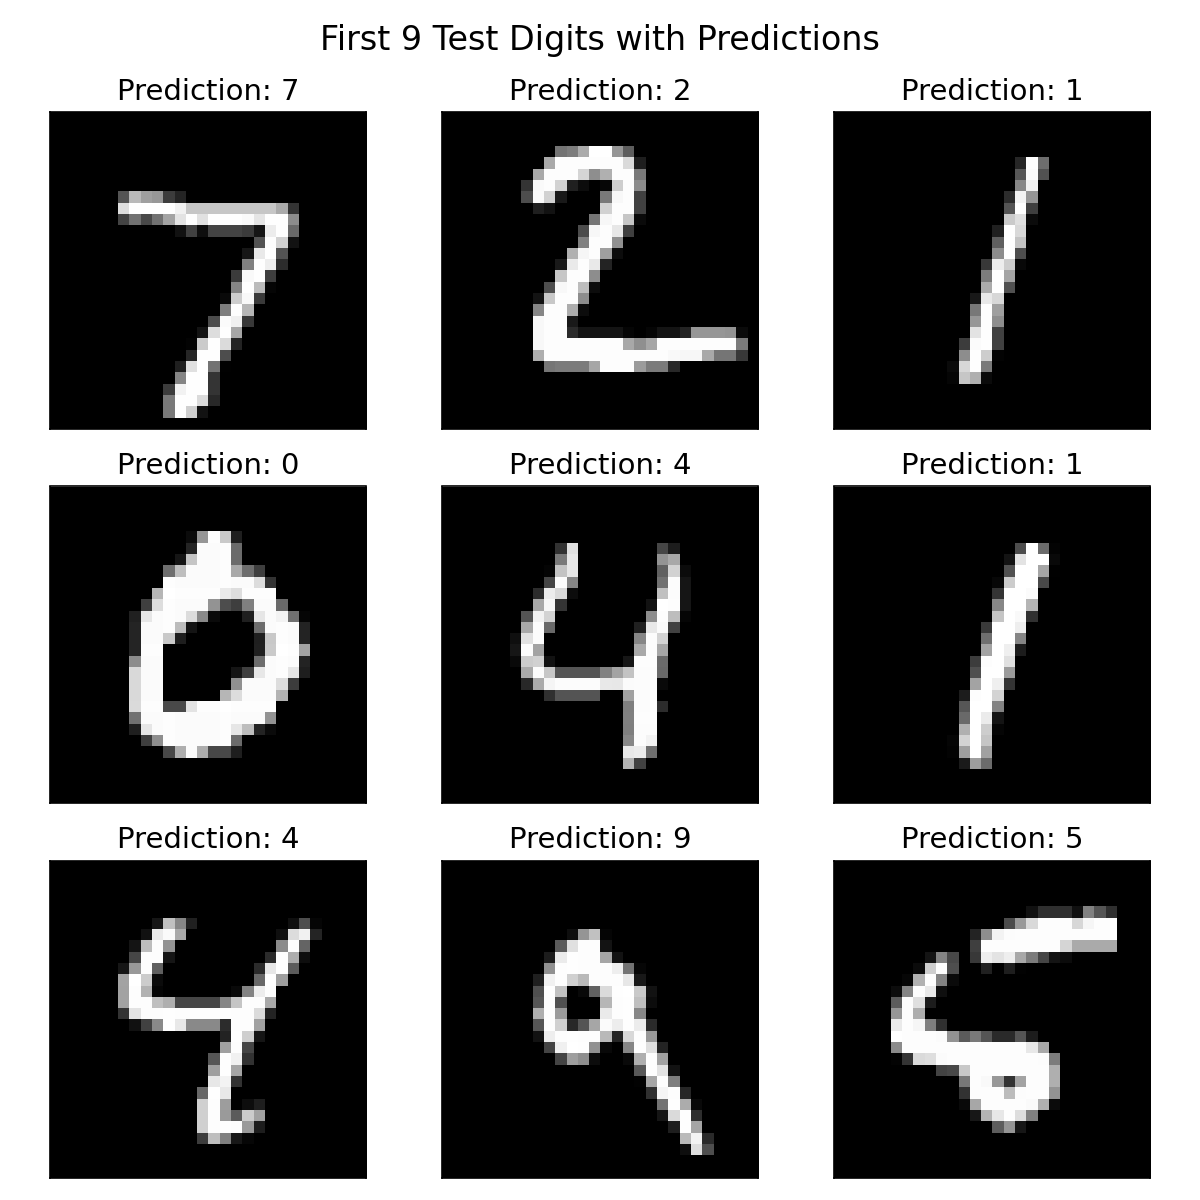
\includegraphics[width=0.55\textwidth]{report_images/test_predictions.png}
    \caption{First 9 test digits in a 3$\times$3 grid with predicted
    labels. Green indicates correct, red indicates misclassification.}
\end{figure}

\subsection{Handwritten Digit Classification}

Digits 0--9 were written by hand with thick marker on white paper,
photographed, and cropped to square images. Preprocessing converts
each to grayscale, resizes to 28$\times$28, inverts intensities (MNIST
uses white-on-black), and normalizes with MNIST statistics
($\mu=0.1307$, $\sigma=0.3081$).

\begin{figure}[H]
    \centering
    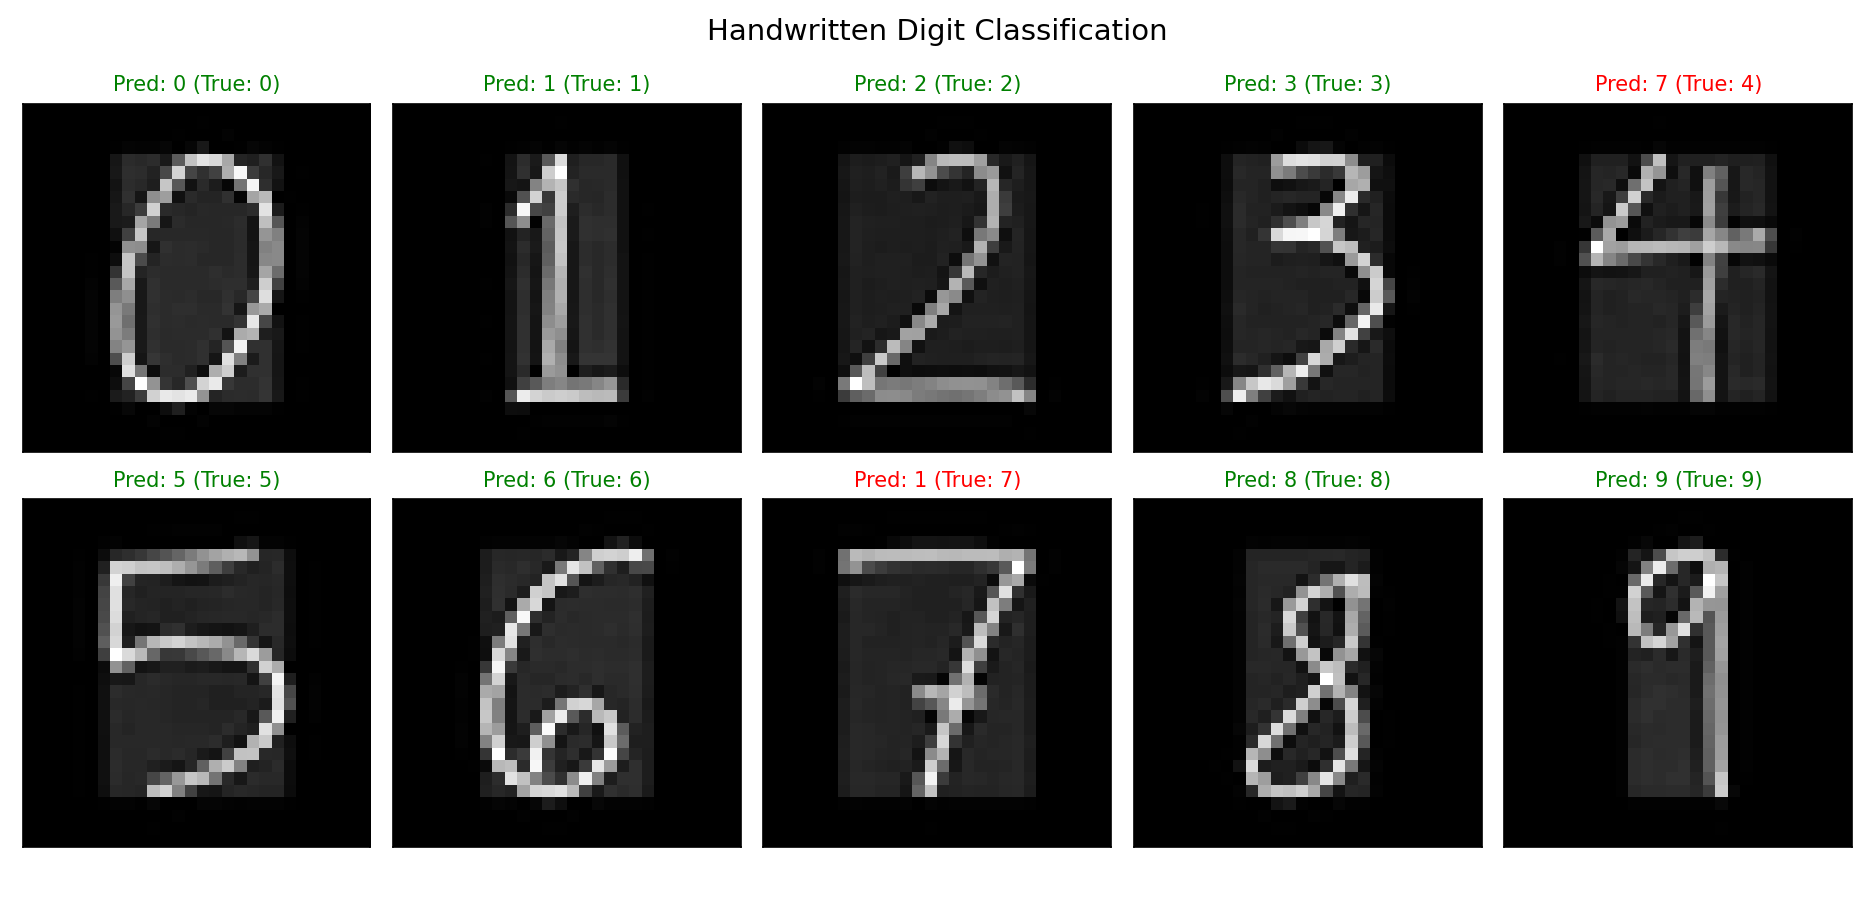
\includegraphics[width=0.7\textwidth]{report_images/handwritten_results.png}
    \caption{Handwritten digits with network predictions. Green
    indicates correct, red indicates misclassification.}
\end{figure}

The network correctly classifies 8 out of 10 handwritten digits.
Two errors occur: digit~4 is predicted as~7, likely because the
angular handwritten strokes of~4 resemble~7, and digit~7 is predicted
as~1, since the simple downstroke of a handwritten~7 without a
crossbar looks like~1. Both errors reflect plausible visual
similarities and are consistent with common MNIST confusions (see
Section~\ref{sec:confusion} for the full confusion matrix analysis on
the test set, which also shows 2$\to$7 as the most frequent error).

% ---------------------------------------------------------------
\section{Task 3 --- Examine Network}
% ---------------------------------------------------------------

\subsection{Model Structure and Weights}

The model structure is:

\begin{verbatim}
MyNetwork(
  (conv1): Conv2d(1, 10, kernel_size=(5, 5), stride=(1, 1))
  (conv2): Conv2d(10, 20, kernel_size=(5, 5), stride=(1, 1))
  (conv2_drop): Dropout2d(p=0.5, inplace=False)
  (fc1): Linear(in_features=320, out_features=50, bias=True)
  (fc2): Linear(in_features=50, out_features=10, bias=True)
)
\end{verbatim}

The first convolutional layer has 10 filters with shape
\texttt{[10, 1, 5, 5]} --- 10 filters, 1 input channel, 5$\times$5
each (250 learnable parameters). All filter weight values were printed
and saved to \texttt{results/examine\_output.txt}. As an example,
Filter~0's learned 5$\times$5 weights are:

\begin{verbatim}
[[-0.12  0.18  0.04  0.23 -0.02]
 [ 0.13 -0.16 -0.19  0.30  0.37]
 [ 0.07 -0.12 -0.20  0.31  0.37]
 [-0.03 -0.03  0.07  0.17  0.02]
 [ 0.09  0.07  0.18 -0.12  0.07]]
\end{verbatim}

\noindent This filter has strong positive values on the right side and
negative values in the center, functioning as a vertical edge detector
--- consistent with its visualization in Figure~\ref{fig:filters}.

\subsection{Filter Visualization}

\begin{figure}[H]
    \centering
    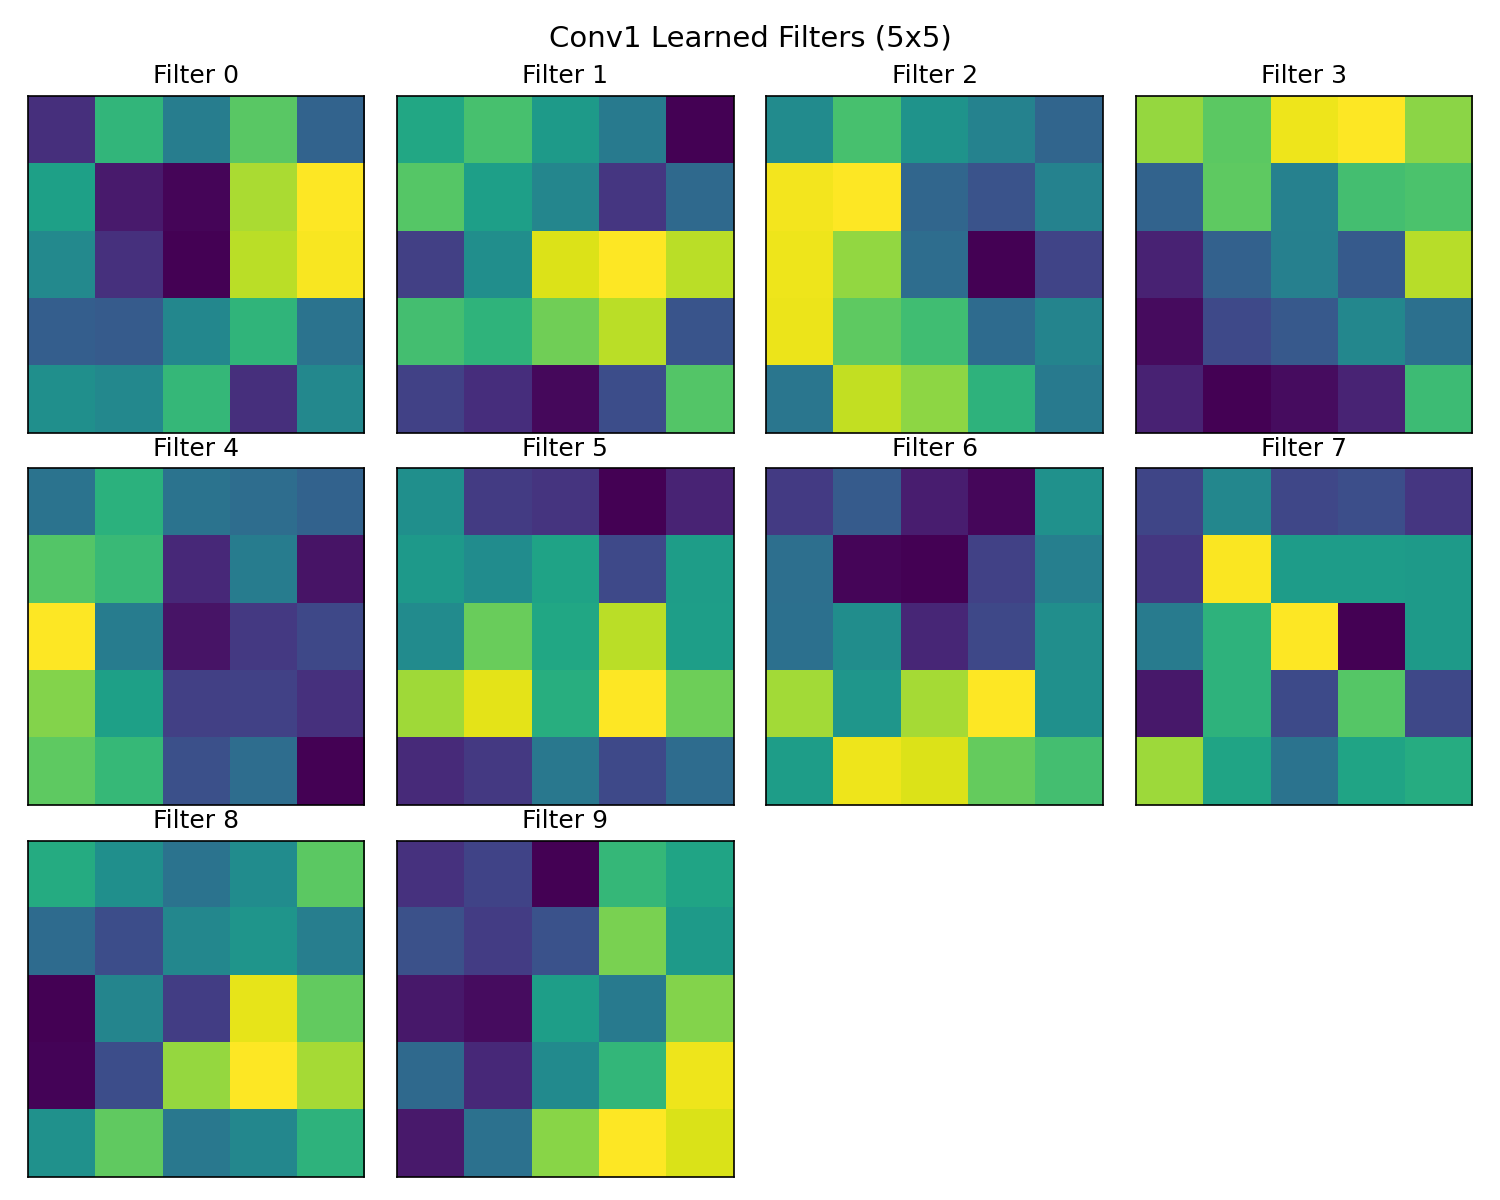
\includegraphics[width=0.6\textwidth]{report_images/conv1_filters.png}
    \caption{The 10 learned 5$\times$5 conv1 filters displayed as
    heatmaps. Several filters resemble oriented edge detectors, while
    others detect corners or texture patterns.}
    \label{fig:filters}
\end{figure}

\subsection{Filter Application}

\begin{figure}[H]
    \centering
    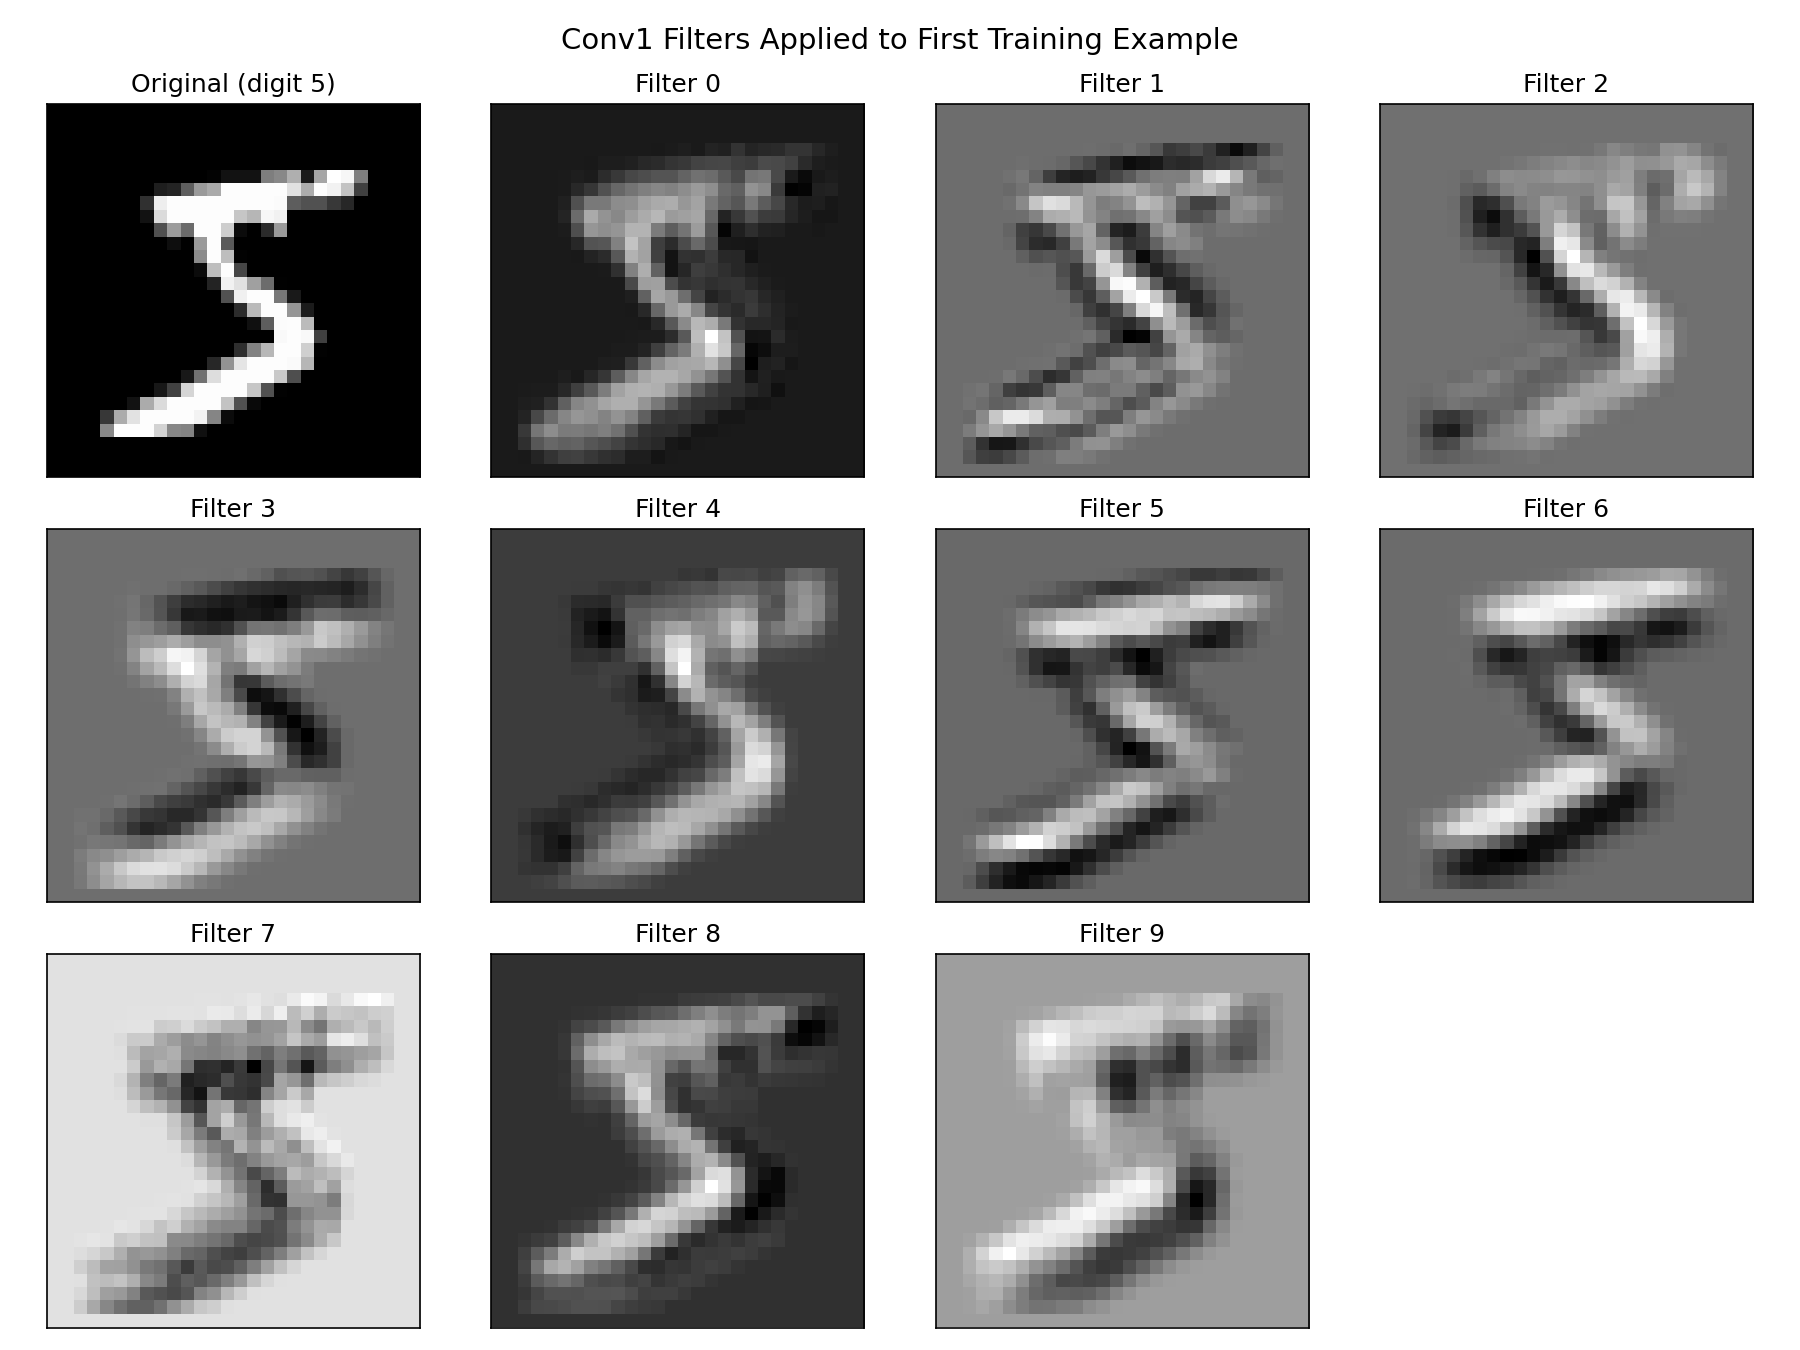
\includegraphics[width=0.7\textwidth]{report_images/conv1_filter_effects.png}
    \caption{Each conv1 filter applied to the first training digit
    via \texttt{cv2.filter2D}. The filtered images highlight edges at
    different orientations, showing how the network decomposes input
    into directional feature maps.}
\end{figure}

\subsection{Analysis}

The filter results align with expectations. Filters with strong
directional gradients act as edge detectors, producing high activation
along edges of that orientation. The variety of orientations ensures
the network detects features at multiple angles, essential for
distinguishing digits like 1 vs 7 or 6 vs 9. These first-layer features
feed into the second convolutional layer, which combines them into
higher-level shape representations.

% ---------------------------------------------------------------
\section{Task 4 --- Transfer Learning on Greek Letters}
% ---------------------------------------------------------------

\subsection{Method}

The pre-trained MNIST network was adapted to classify Greek letters
via transfer learning. All parameters were frozen and \texttt{fc2} was
replaced with a new classification layer. For the base 3-class task
(alpha, beta, gamma), \texttt{fc2} was set to \texttt{Linear(50, 3)}
and trained on the 27 provided course examples, reaching 100\%
training accuracy within 15 epochs. As an extension, 3 additional
classes were added (delta, epsilon, lambda) with user-drawn examples,
replacing \texttt{fc2} with \texttt{Linear(50, 6)} and bringing the
total to 6 classes and 60 training images. The remainder of this
section reports results for the full 6-class system.
The modified network structure:

\begin{verbatim}
MyNetwork(
  (conv1): Conv2d(1, 10, kernel_size=(5, 5), stride=(1, 1))
  (conv2): Conv2d(10, 20, kernel_size=(5, 5), stride=(1, 1))
  (conv2_drop): Dropout2d(p=0.5, inplace=False)
  (fc1): Linear(in_features=320, out_features=50, bias=True)
  (fc2): Linear(in_features=50, out_features=6, bias=True)
)
\end{verbatim}

The only change is the final layer: 50$\to$6 instead of 50$\to$10.
The \texttt{GreekTransform} pipeline converts color images to MNIST
format: grayscale, affine scale (36/128), center crop (28$\times$28),
and intensity inversion.

Training used SGD (lr=0.01, momentum=0.9) on \texttt{fc2} parameters
only, with batch size 5 and early stopping at 100\% training accuracy.
The model required 37 epochs to reach 100\% on the 60-image training
set.

\subsection{Training Results}

\begin{figure}[H]
    \centering
    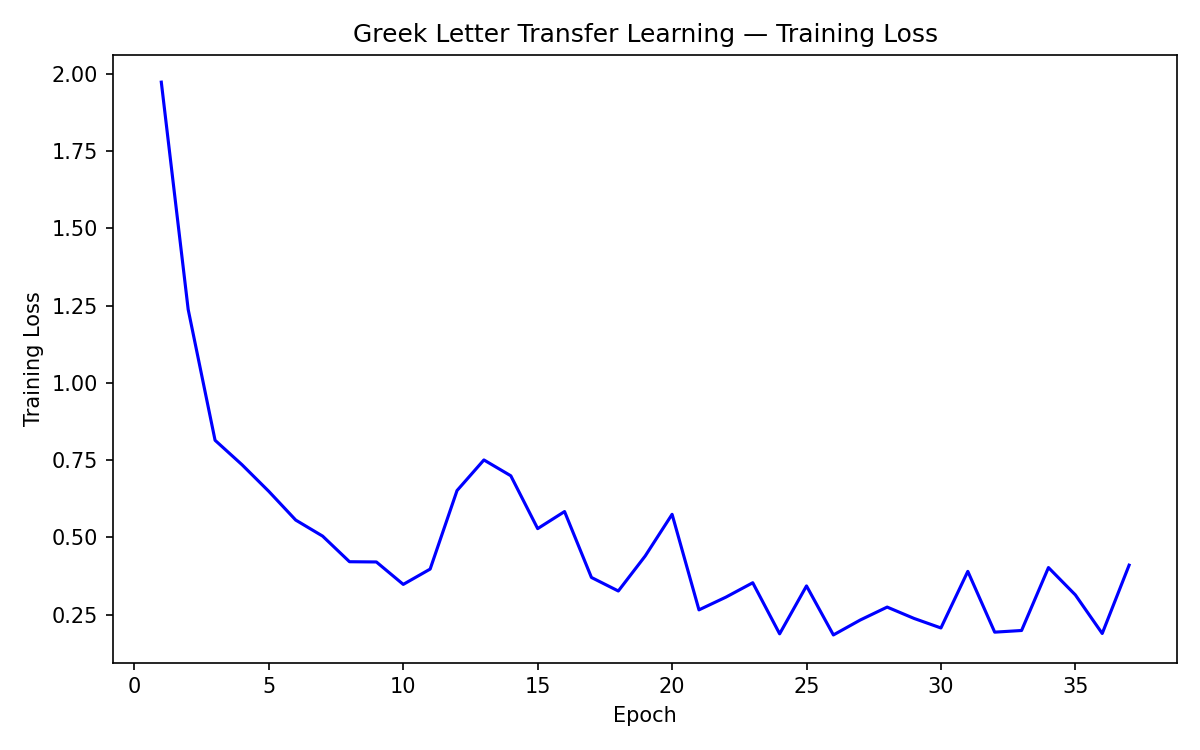
\includegraphics[width=0.6\textwidth]{report_images/greek_training_loss.png}
    \caption{Training loss for Greek letter transfer learning. The
    oscillation reflects the extremely small dataset (60 images, batch
    size 5).}
\end{figure}

\subsection{Test Results}

\begin{figure}[H]
    \centering
    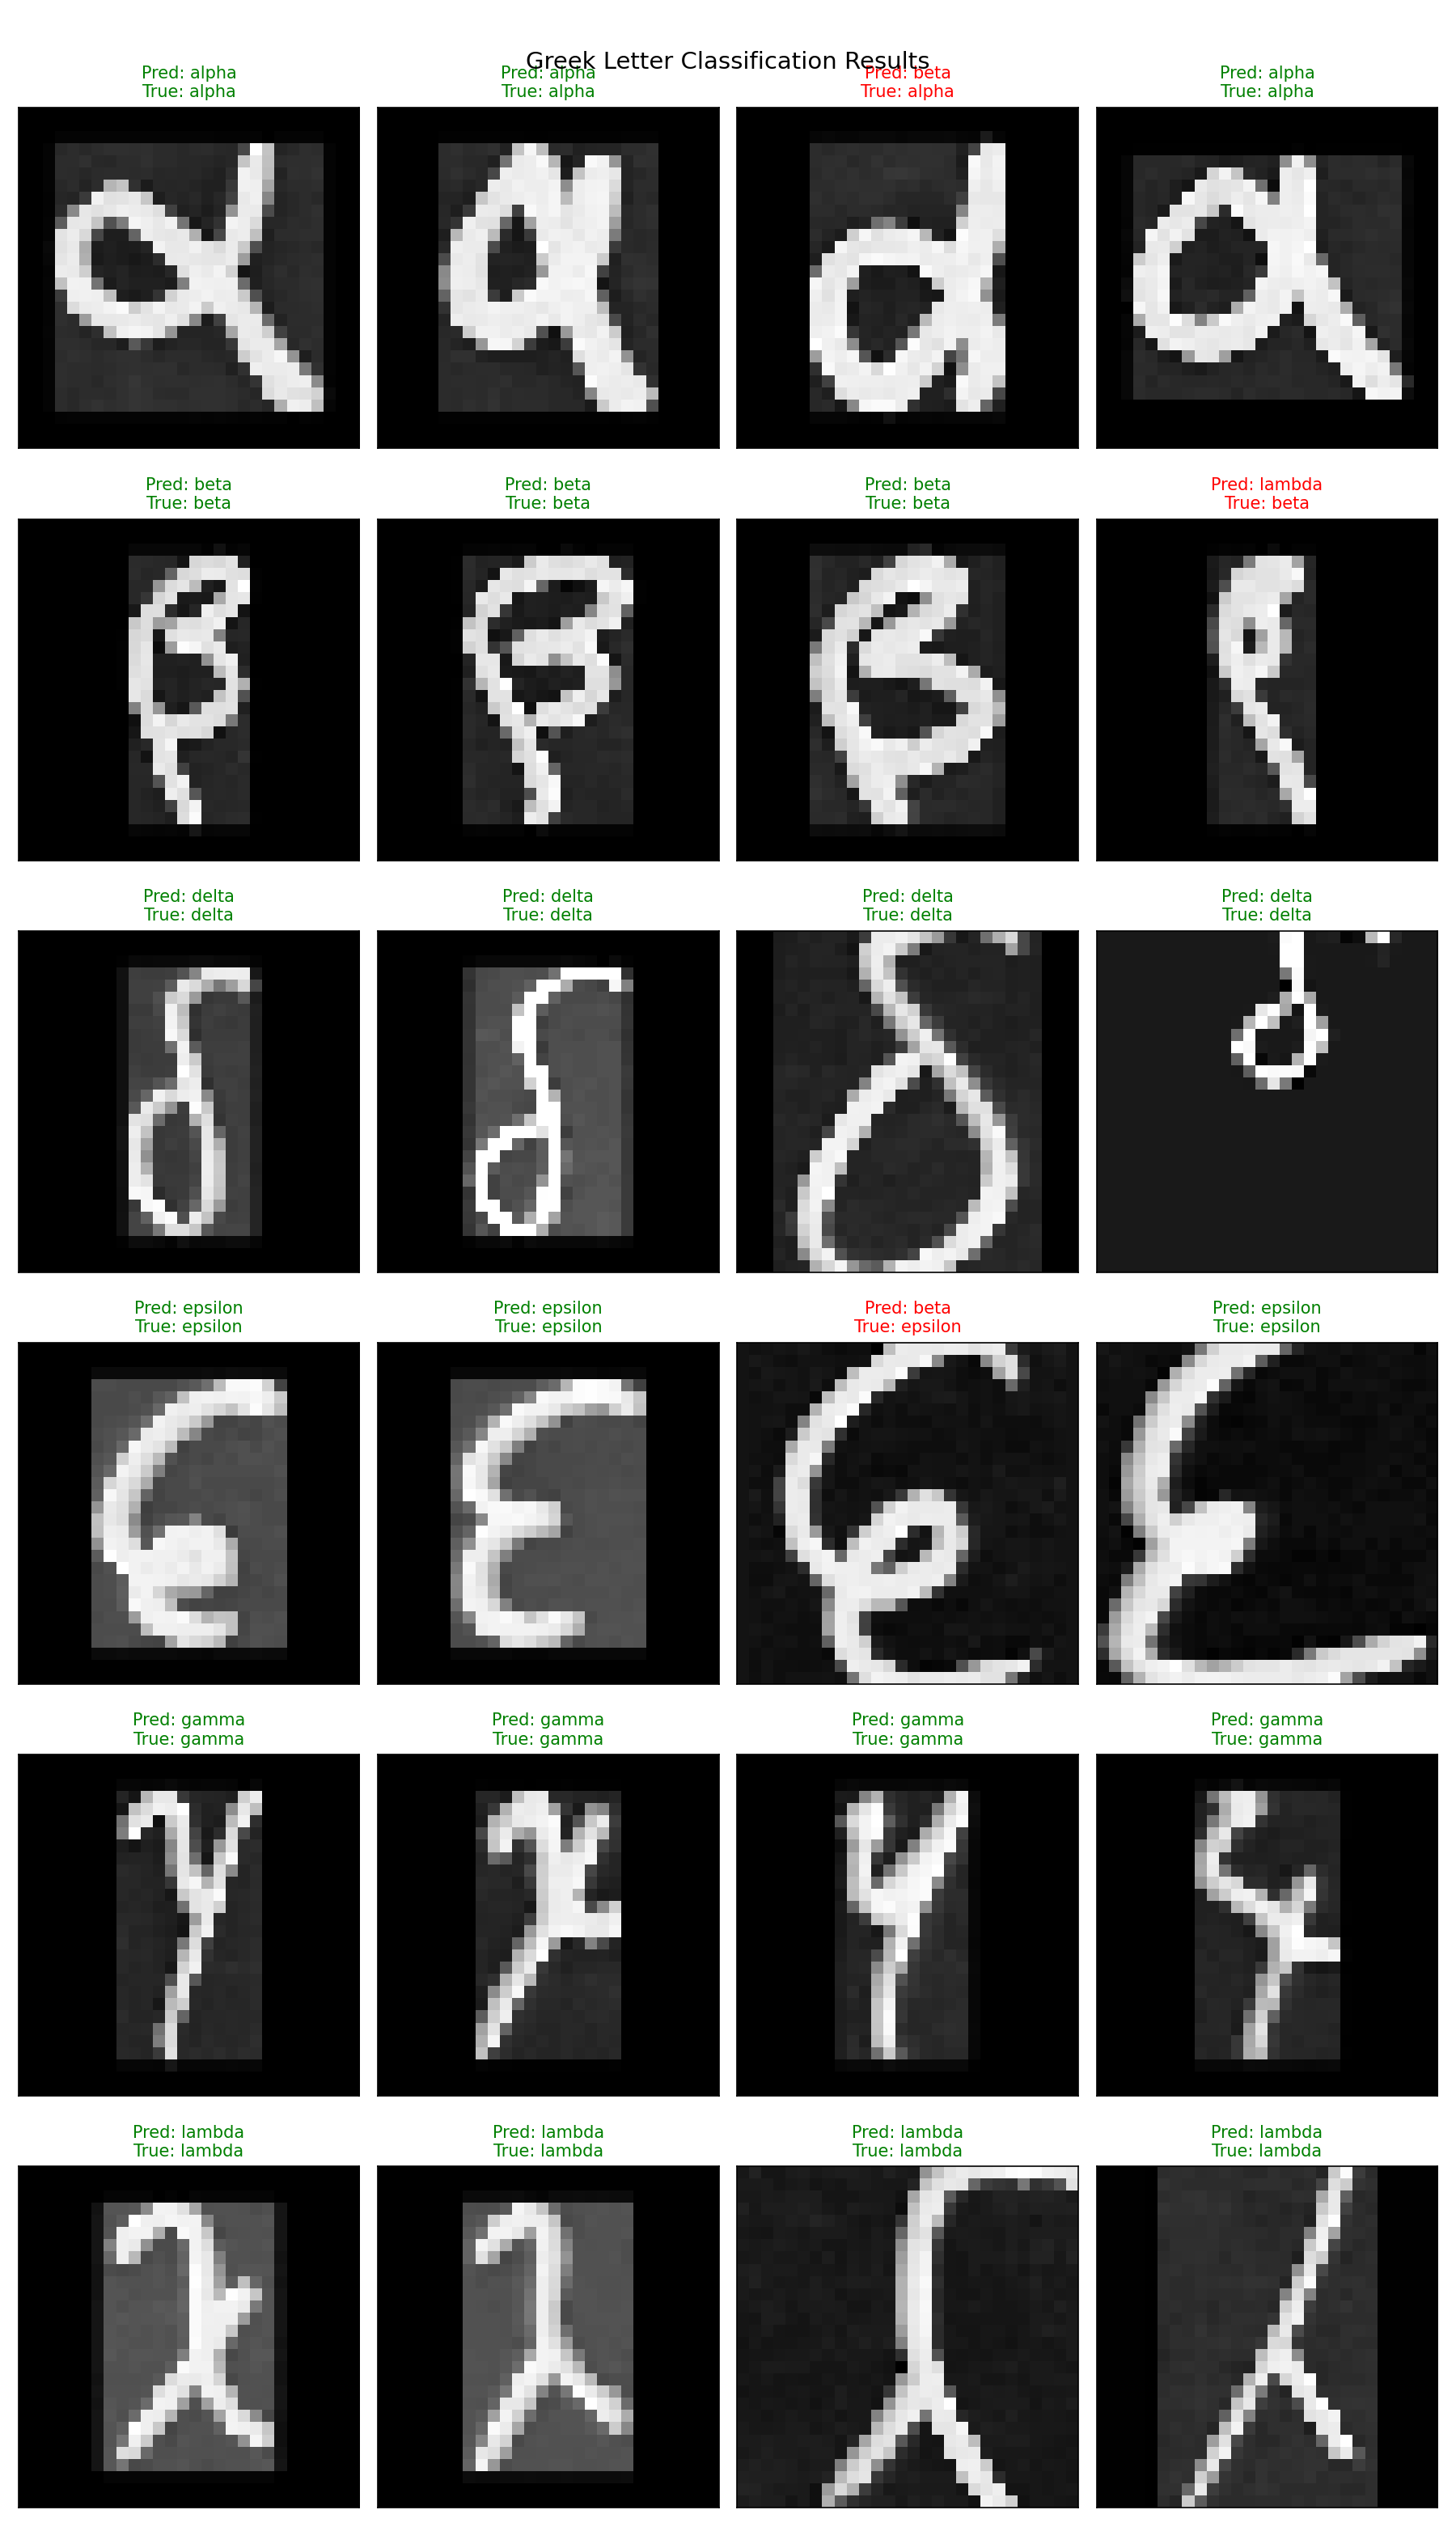
\includegraphics[width=0.55\textwidth]{report_images/greek_test_results.png}
    \caption{Classification results on 24 Greek letter test images.
    Green titles indicate correct predictions, red indicates errors.
    The model achieves 88\% accuracy (21/24).}
\end{figure}

\subsection{Iterative Improvement Process}

Initial accuracy was approximately 40\%. Systematic investigation
revealed the root cause: the provided alpha/beta/gamma training images
(thin pencil strokes from the course dataset) looked fundamentally
different from the user's test images (thick marker on white paper)
after preprocessing. The model had never seen thick-stroke examples
for these three classes.

A diagnostic test confirmed this: a 3-class model trained on only the
provided alpha/beta/gamma images achieved just 25\% on user-drawn test
images, despite reaching 100\% on the thin-stroke training data.

A tuning script (\texttt{greek\_tuner.py}) was developed to
systematically test 10 configurations across three freeze levels
(fc2-only, fc1+fc2, all layers), two optimizers (SGD, Adam), and
multiple learning rates. This replaced ad-hoc manual experimentation.
Table~\ref{tab:tuner} shows the ranked results.

\begin{table}[H]
    \centering
    \begin{tabular}{llrl}
        \toprule
        Freeze Level & Optimizer & Accuracy & Epochs \\
        \midrule
        fc2-only  & SGD lr=0.01           & \textbf{87.5\%} & 30 \\
        fc1+fc2   & SGD lr=0.01           & 83.3\% & 5 \\
        all       & SGD lr=0.001          & 83.3\% & 10 \\
        fc2-only  & Adam lr=0.001         & 79.2\% & 57 \\
        fc1+fc2   & Adam lr=0.001         & 79.2\% & 6 \\
        fc1+fc2   & Adam lr=0.0005 wd=1e-4 & 79.2\% & 10 \\
        all       & SGD lr=0.005          & 79.2\% & 9 \\
        all       & Adam lr=0.0005 wd=1e-4 & 79.2\% & 5 \\
        all       & Adam lr=0.0001        & 75.0\% & 28 \\
        all       & Adam lr=0.0005        & 75.0\% & 10 \\
        \bottomrule
    \end{tabular}
    \caption{Greek letter tuning results ranked by test accuracy.
    fc2-only SGD achieved the highest accuracy at 87.5\% and was
    selected for the final model as the simplest effective configuration.}
    \label{tab:tuner}
\end{table}

The key terms:
\begin{itemize}
    \item \textbf{fc2-only:} freeze the entire pretrained network,
    train only the final 50$\to$6 linear classifier. Simplest but
    least flexible.
    \item \textbf{fc1+fc2:} also unfreeze the hidden layer
    (320$\to$50), allowing intermediate feature adaptation.
    \item \textbf{All unfrozen:} convolutional layers adapt too,
    giving maximum flexibility but risking overfitting on 60 images.
\end{itemize}

The fix was twofold: (1) the provided alpha/beta/gamma training images
were preprocessed with a PIL \texttt{MinFilter(5)} morphological
operation to thicken their thin pencil strokes, better matching the
style of user-drawn test images; and (2) 2 user-drawn images per class
were added to the alpha/beta/gamma training data, giving the model
direct exposure to the thick-stroke style. Together these changes raised
accuracy from approximately 40\% to 83--88\%. Moving more test images to training was considered but
rejected because it would leave only 1 test image per class,
making evaluation unreliable.

The final train/test split:

\begin{table}[H]
    \centering
    \begin{tabular}{lccccc}
        \toprule
        Class & Provided Train & User Train & Total Train & User Test \\
        \midrule
        alpha   & 9 & 2 & 11 & 4 \\
        beta    & 9 & 2 & 11 & 4 \\
        gamma   & 9 & 2 & 11 & 4 \\
        delta   & 0 & 9 &  9 & 4 \\
        epsilon & 0 & 9 &  9 & 4 \\
        lambda  & 0 & 9 &  9 & 4 \\
        \midrule
        Total   & 27 & 33 & 60 & 24 \\
        \bottomrule
    \end{tabular}
    \caption{Train/test split for Greek letter classification. Adding
    user-drawn images to alpha/beta/gamma training was the key to
    resolving the domain shift.}
\end{table}

\textbf{Known limitation:} Several user-drawn images for delta, epsilon,
and lambda were initially saved with incorrect rotation due to photo
orientation metadata not being preserved during cropping. This was
identified and corrected, though the small dataset size (60 train, 24
test) means individual image quality variations still have outsized
impact on accuracy.

\textbf{Key lesson:} Transfer learning on tiny datasets is extremely
sensitive to domain shift between training and test images. The MNIST
features transfer well, but the classifier layer can only succeed if
train and test images look similar after preprocessing.

% ---------------------------------------------------------------
\section{Task 5 --- Transformer Re-implementation}
% ---------------------------------------------------------------

\subsection{Method}

A vision transformer was implemented following the provided template.
The forward pass consists of five steps: patch embedding, positional
embedding addition, dropout, transformer encoder (multi-head
self-attention + feedforward), and layer normalization followed by
classification. Default configuration: patch size 4, stride 2,
embedding dimension 48, depth 4, 8 attention heads, MLP dimension 128,
15 epochs.

\subsection{Results}

\begin{figure}[H]
    \centering
    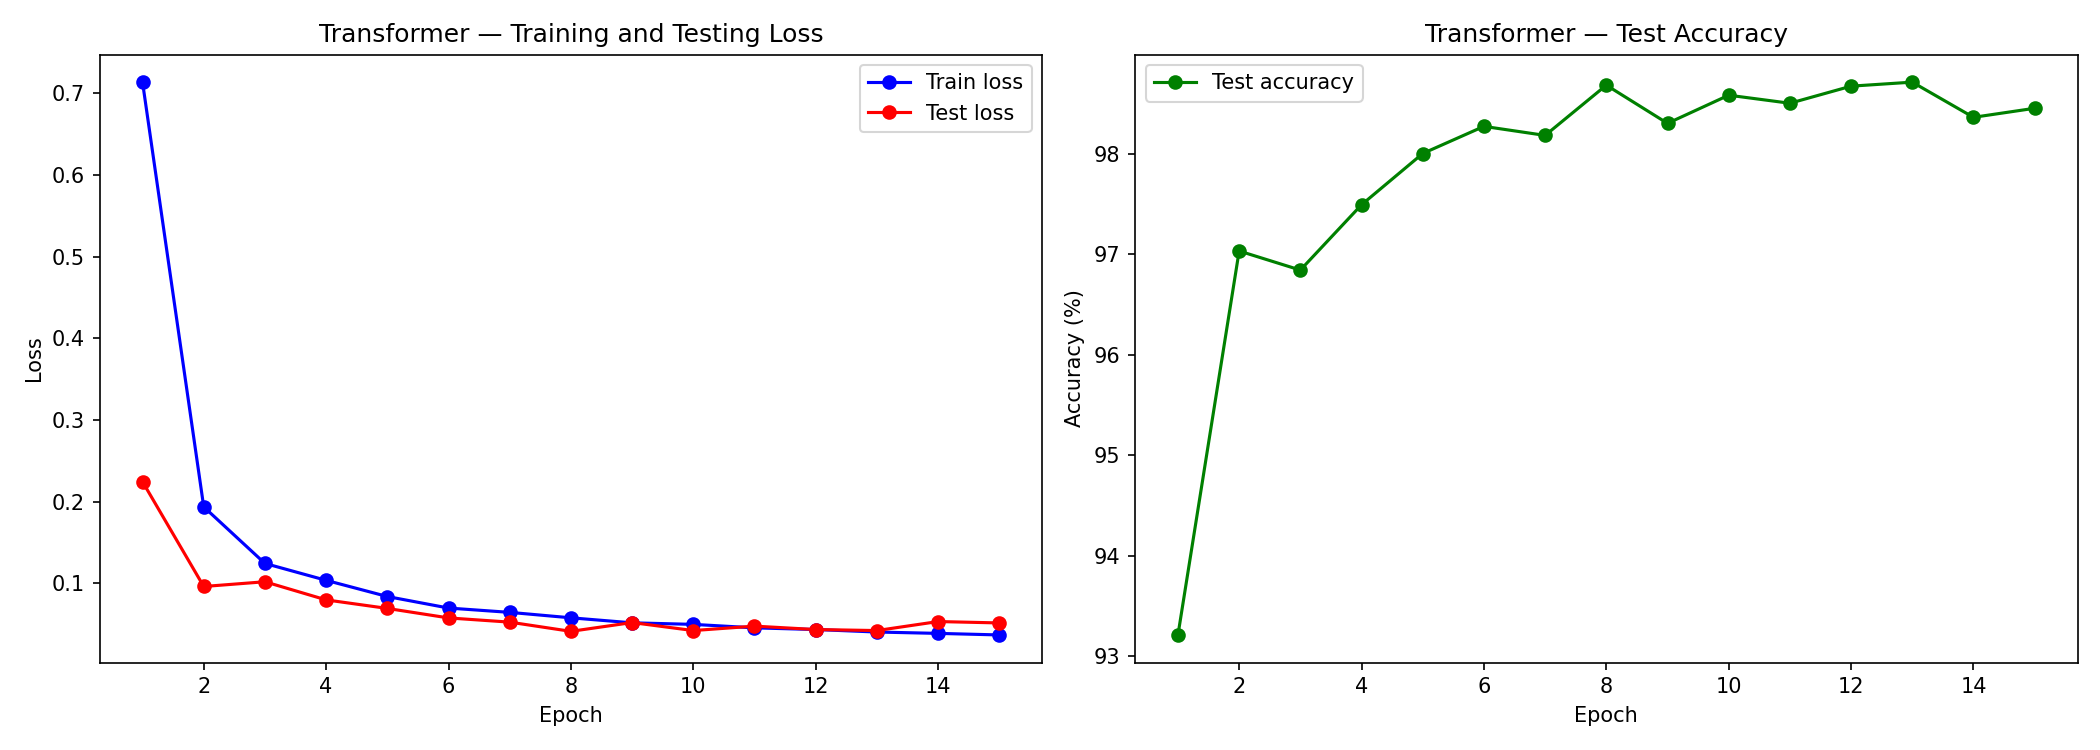
\includegraphics[width=0.7\textwidth]{report_images/transformer_results.png}
    \caption{Transformer training results: loss curve and accuracy
    curve across 15 epochs.}
\end{figure}

\begin{table}[H]
    \centering
    \begin{tabular}{lccc}
        \toprule
        Model & Best Test Acc & Final Test Acc & Training Time \\
        \midrule
        CNN (5 epochs) & 98.00\% & 97.93\% & $\sim$2 min \\
        Transformer (15 epochs) & 98.71\% & 98.45\% & $\sim$90 min \\
        \bottomrule
    \end{tabular}
    \caption{CNN vs Transformer comparison on MNIST. The transformer
    slightly outperforms but requires significantly more computation.}
\end{table}

The transformer slightly outperforms the CNN in accuracy but trains
roughly 45$\times$ slower. On a small 28$\times$28 dataset like MNIST,
the CNN's inductive bias (translation equivariance, local receptive
fields) makes it far more data-efficient, while the transformer's
self-attention mechanism needs more computation to learn spatial
relationships from scratch.

% ---------------------------------------------------------------
\section{Task 6 --- Architecture Experiment on Fashion MNIST}
% ---------------------------------------------------------------

\subsection{Experiment Plan}

\textbf{Dataset:} Fashion MNIST (10 clothing categories, 60k train /
10k test, 28$\times$28 grayscale). Chosen over MNIST digits because
it is more challenging and provides more room to observe architectural
effects.

\textbf{Three dimensions explored:}
\begin{enumerate}
    \item Number of convolution filters (conv1/conv2):
    [4, 8, 16, 24, 32, 48, 64, 96, 128]
    \item Dropout rate: [0.0, 0.1, 0.2, 0.3, 0.4, 0.5, 0.6, 0.7]
    \item Hidden FC nodes: [16, 32, 64, 128, 192, 256, 384, 512]
\end{enumerate}

\textbf{Strategy:} Two-round linear search---sweep one dimension while
holding others at baseline, update baseline with best value, repeat.
Total: 50 configurations ($[9{+}8{+}8] \times 2$ rounds), 5 epochs
each. A full grid search ($9 \times 8 \times 8 = 576$ configs) would
take approximately 8 hours; the linear search captures key trends in
approximately 79 minutes on M1 MPS.

\subsection{Hypotheses}

\begin{enumerate}
    \item \textbf{Conv filters:} Accuracy will increase up to
    $\sim$32--48 filters then plateau. Fashion MNIST's visual complexity
    at 28$\times$28 is limited. Training time should scale linearly.

    \item \textbf{Dropout:} Moderate dropout (0.2--0.3) will perform
    best. Zero dropout will overfit; high dropout ($>$0.5) will
    underfit by discarding too much information.

    \item \textbf{Hidden nodes:} Accuracy will improve from 16 to
    $\sim$128--256 then plateau. Too few nodes bottleneck the classifier;
    too many add parameters without benefit.
\end{enumerate}

\subsection{Results}

\begin{figure}[H]
    \centering
    \begin{subfigure}[b]{0.48\textwidth}
        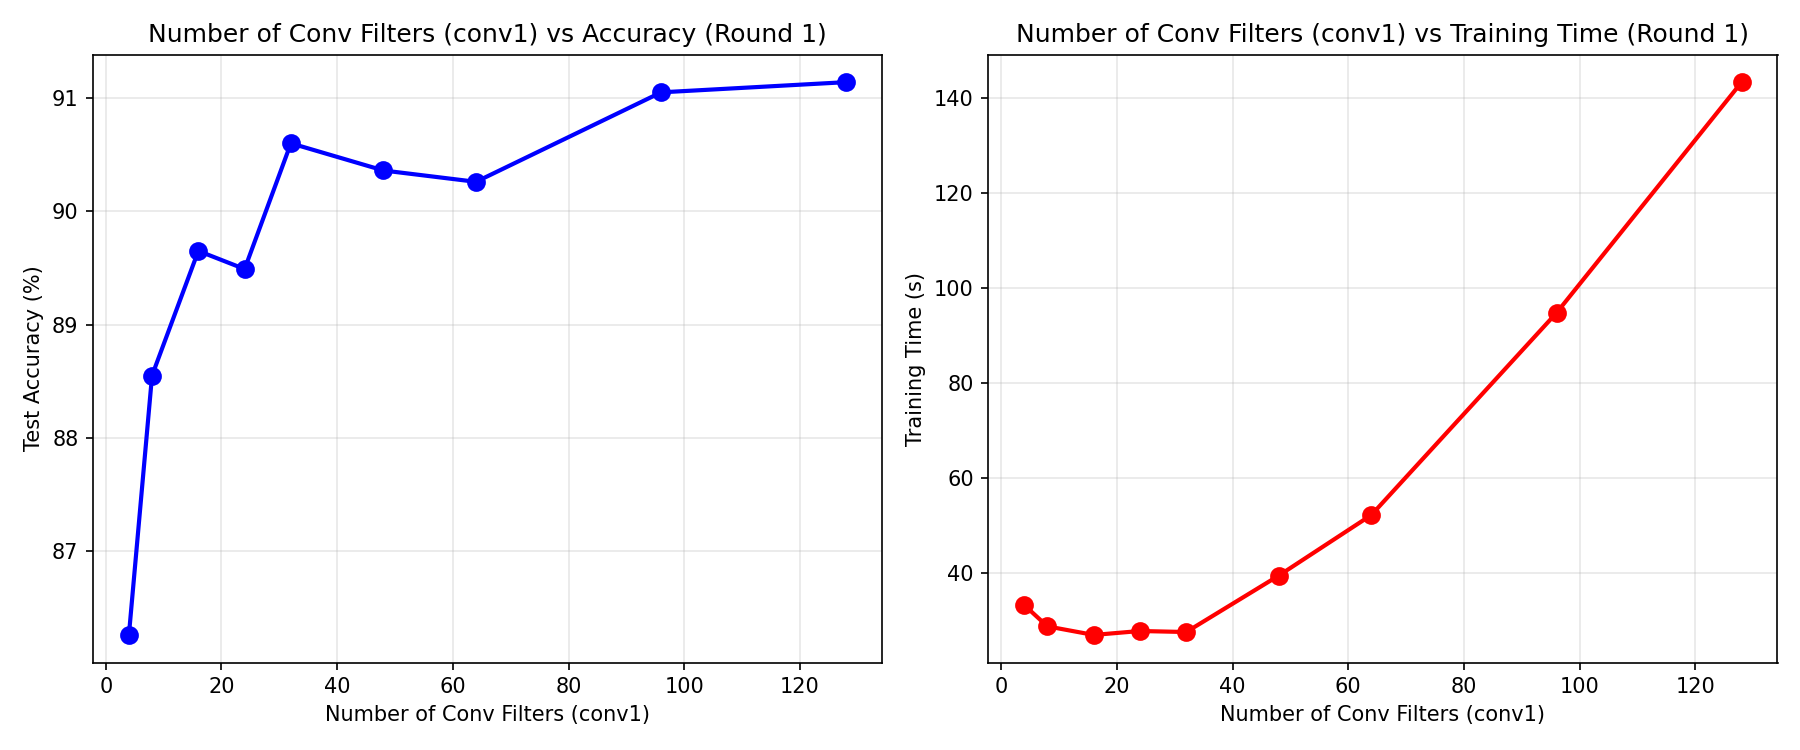
\includegraphics[width=\textwidth]{report_images/experiment_conv1_filters_round1.png}
        \caption{Conv filters --- Round 1}
    \end{subfigure}
    \hfill
    \begin{subfigure}[b]{0.48\textwidth}
        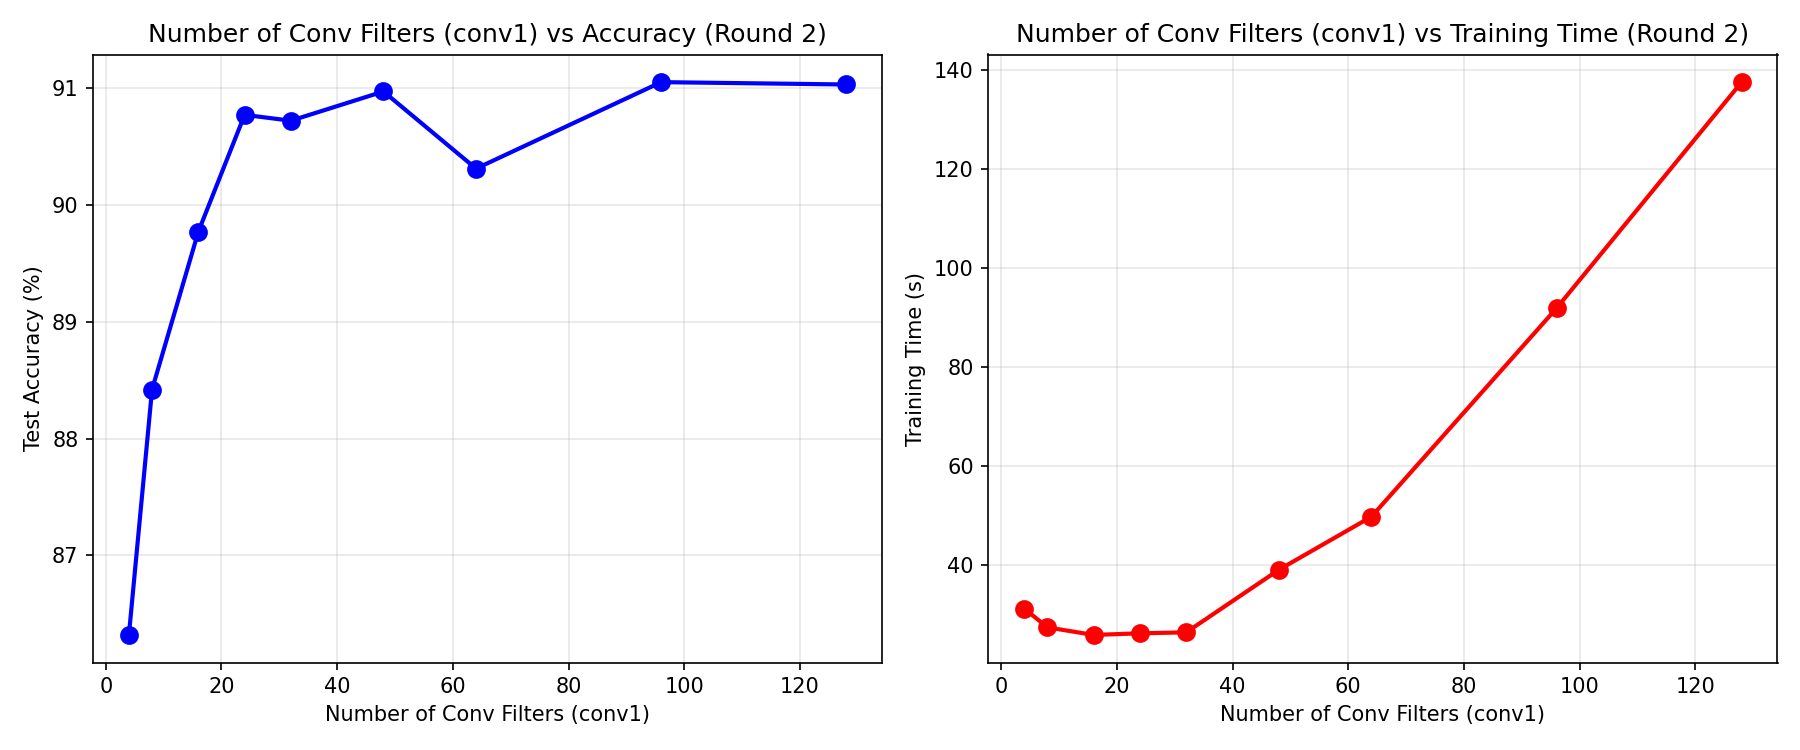
\includegraphics[width=\textwidth]{report_images/experiment_conv1_filters_round2.png}
        \caption{Conv filters --- Round 2}
    \end{subfigure}

    \vspace{0.5em}
    \begin{subfigure}[b]{0.48\textwidth}
        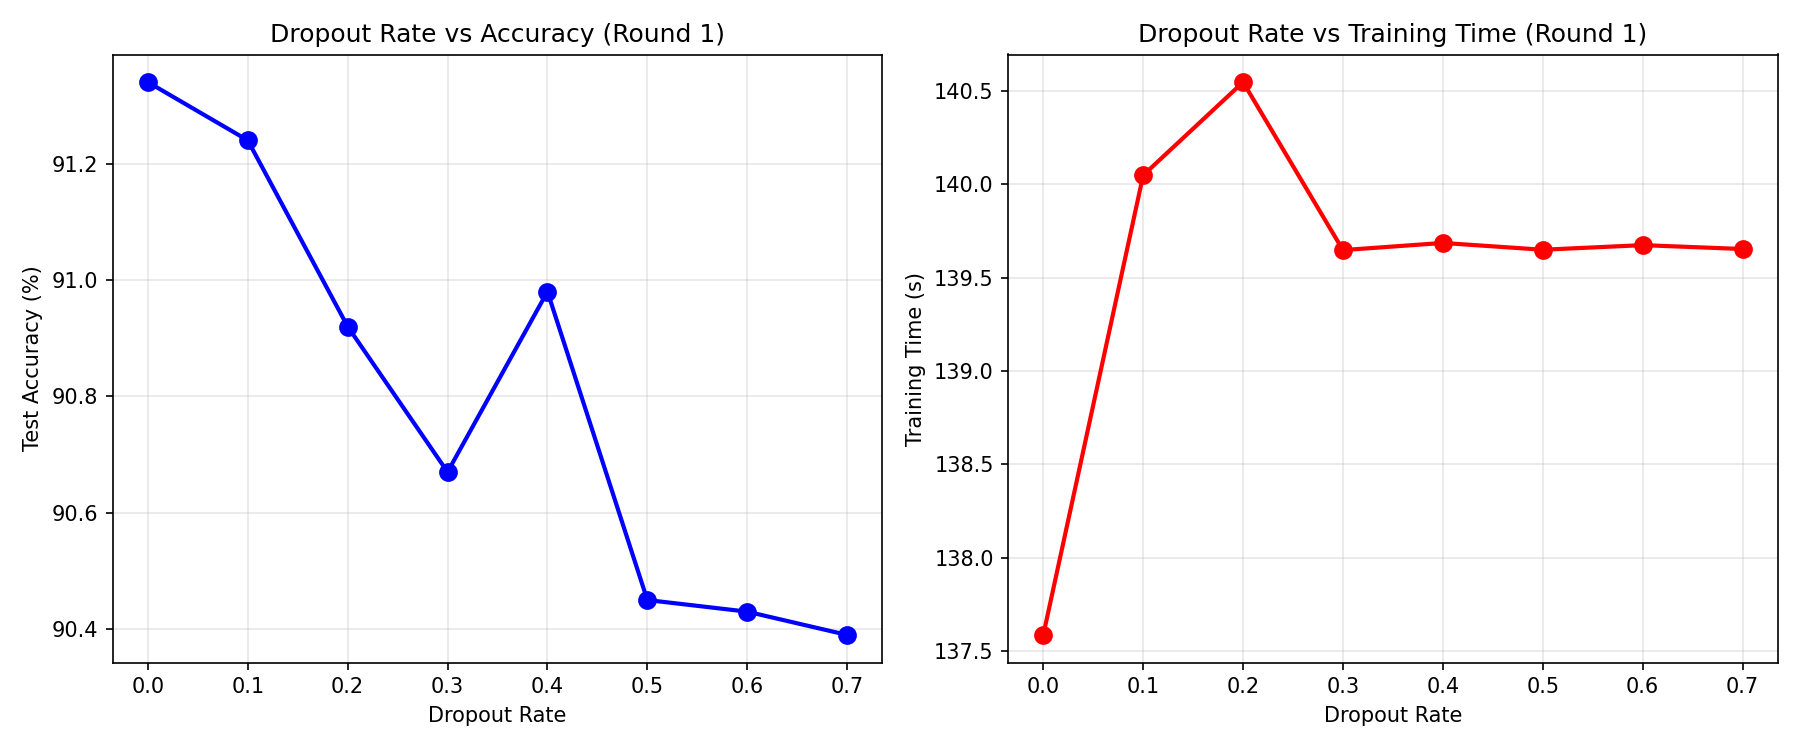
\includegraphics[width=\textwidth]{report_images/experiment_dropout_rate_round1.png}
        \caption{Dropout --- Round 1}
    \end{subfigure}
    \hfill
    \begin{subfigure}[b]{0.48\textwidth}
        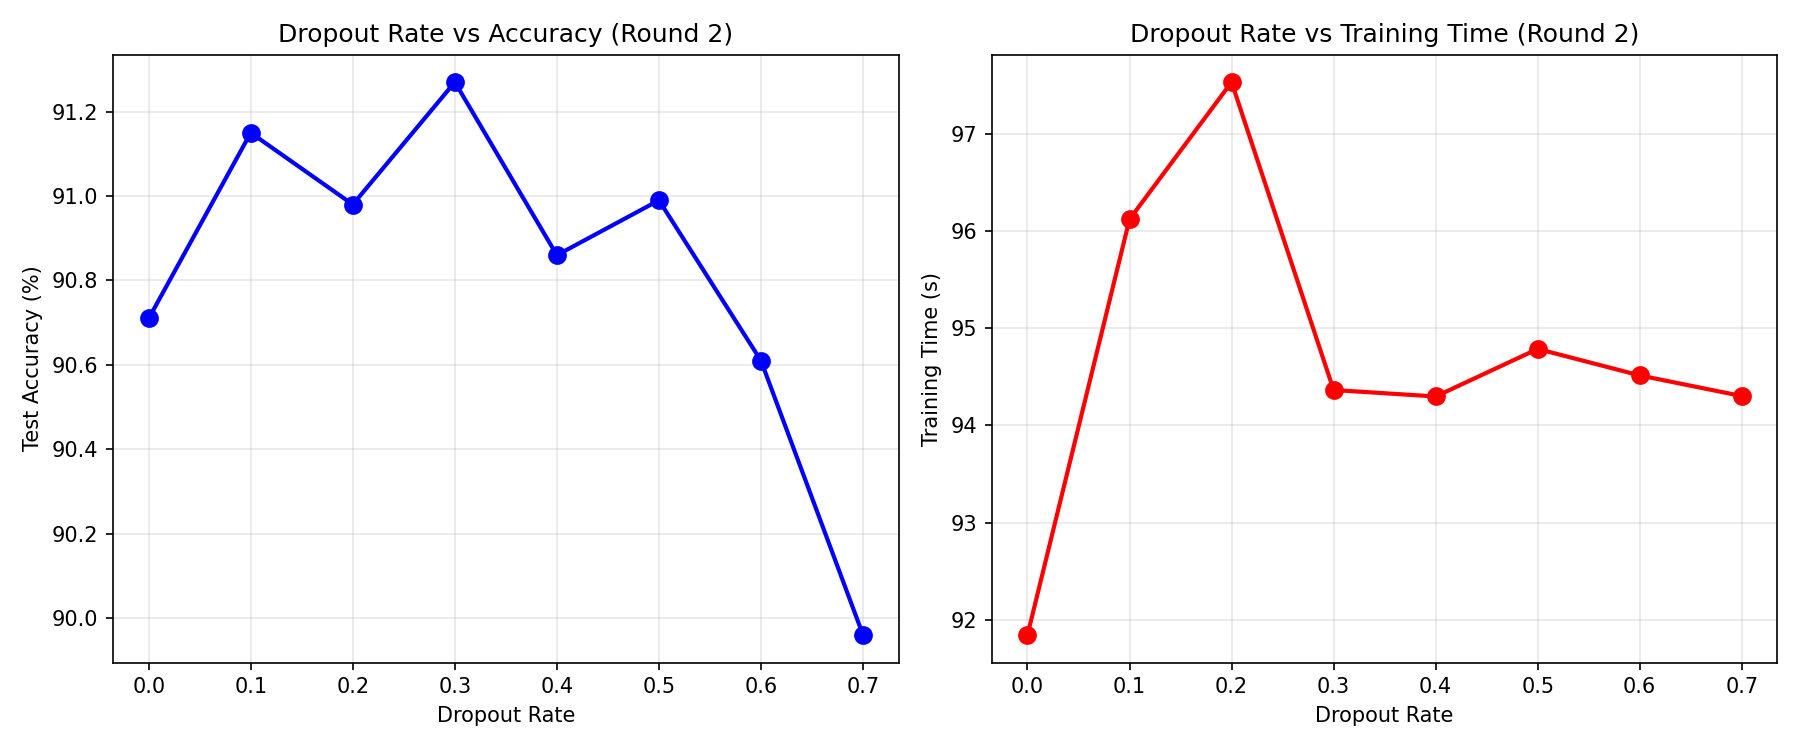
\includegraphics[width=\textwidth]{report_images/experiment_dropout_rate_round2.png}
        \caption{Dropout --- Round 2}
    \end{subfigure}

    \vspace{0.5em}
    \begin{subfigure}[b]{0.48\textwidth}
        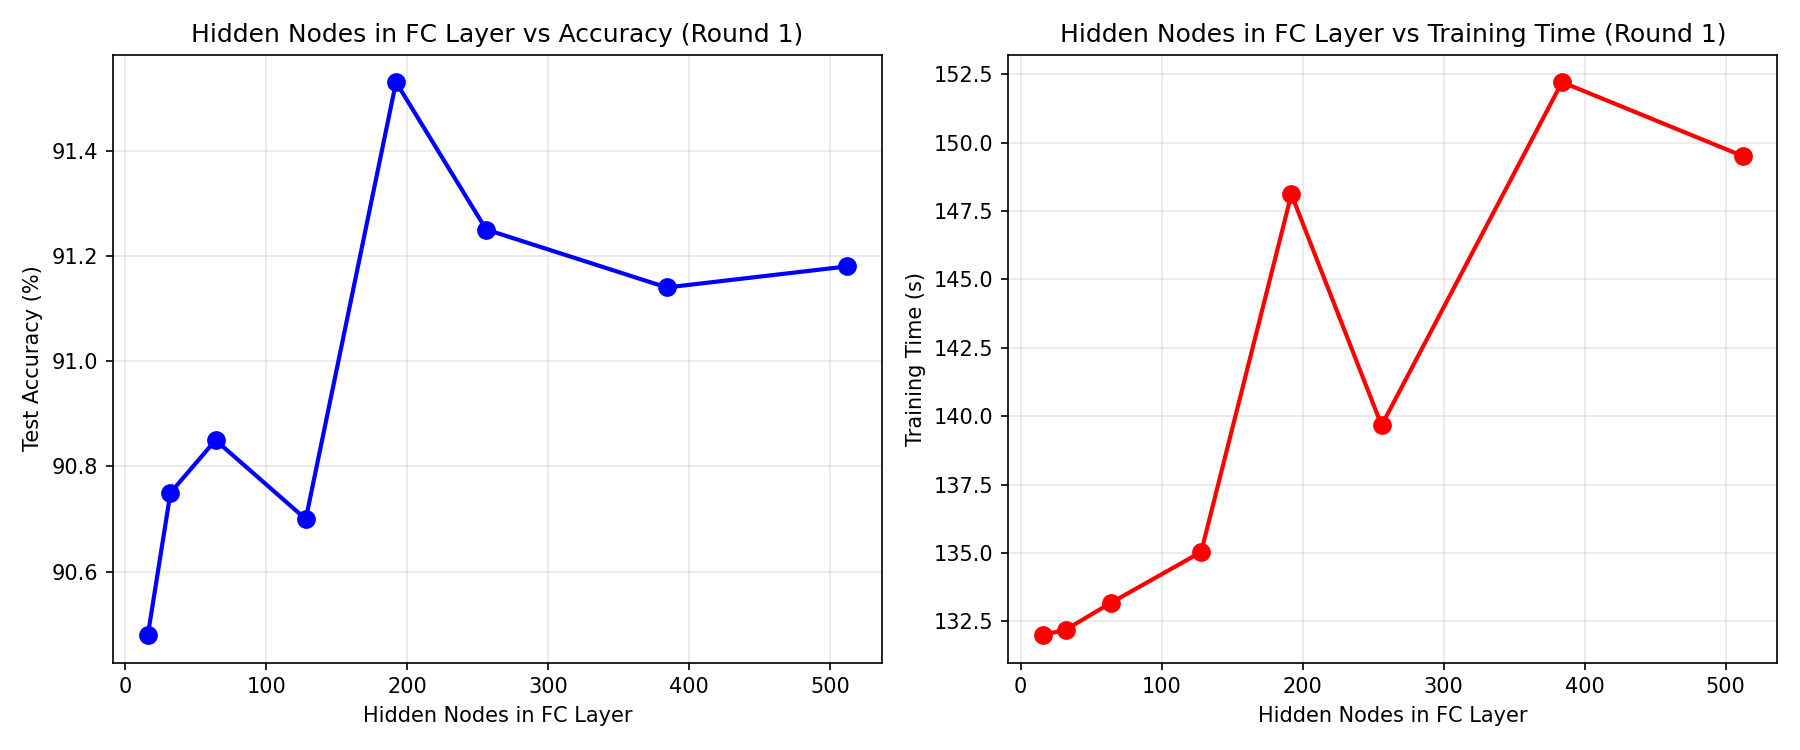
\includegraphics[width=\textwidth]{report_images/experiment_hidden_nodes_round1.png}
        \caption{Hidden nodes --- Round 1}
    \end{subfigure}
    \hfill
    \begin{subfigure}[b]{0.48\textwidth}
        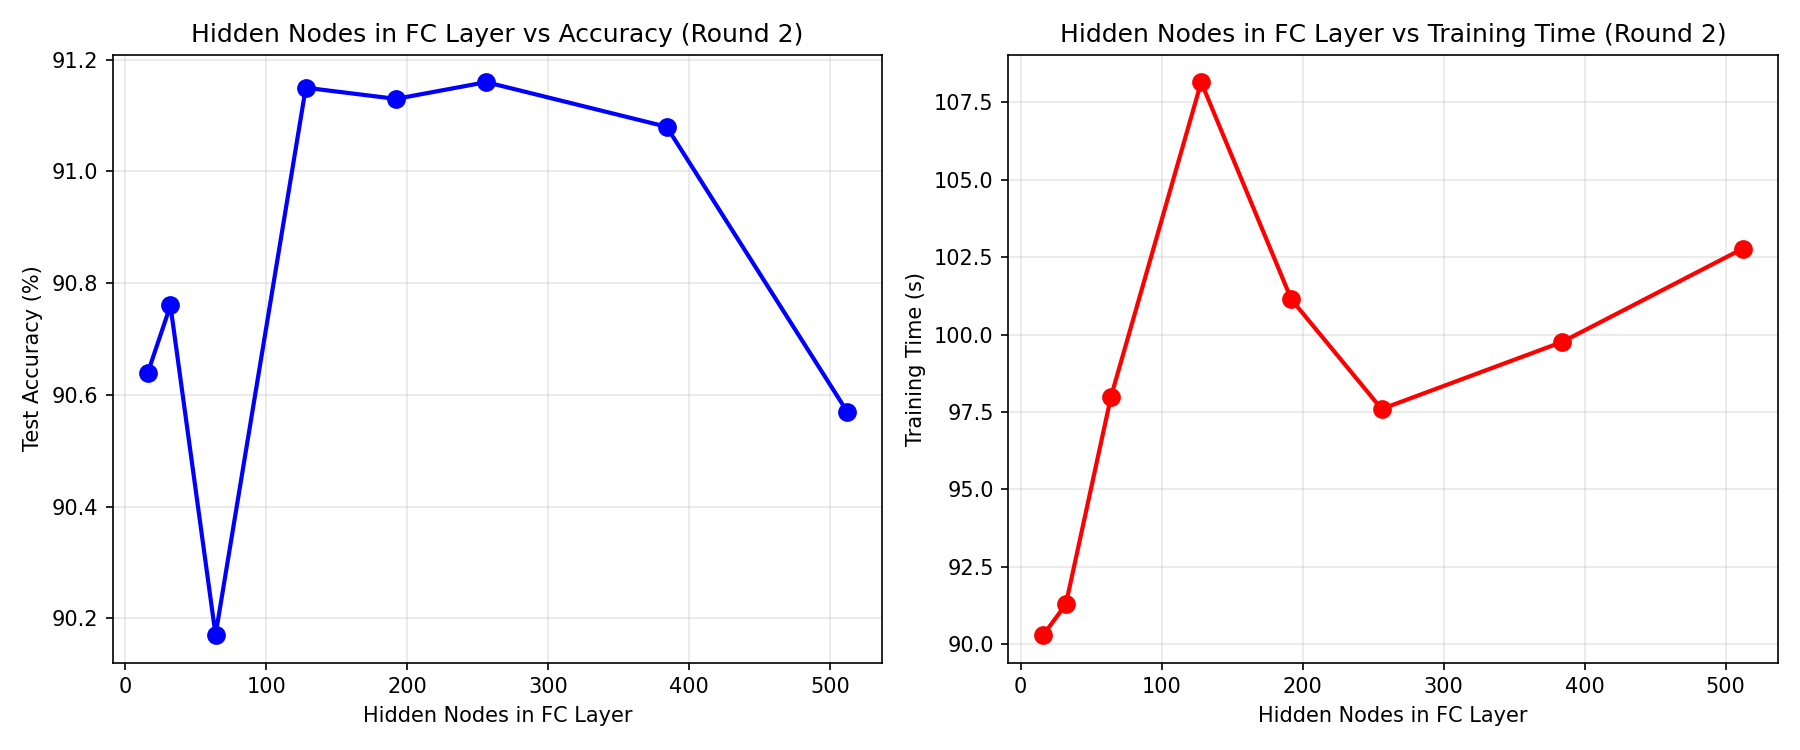
\includegraphics[width=\textwidth]{report_images/experiment_hidden_nodes_round2.png}
        \caption{Hidden nodes --- Round 2}
    \end{subfigure}
    \caption{Accuracy and training time vs each architectural dimension
    across two rounds of linear search. Best configuration: conv1=96,
    conv2=192, dropout=0.3, hidden=256 (91.53\% peak).}
\end{figure}

\subsection{Discussion: Hypotheses vs Results}

\textbf{Conv filters (partially supported):} Predicted plateau at
32--48; actual plateau closer to 96. Fashion MNIST benefits from more
filters than expected---clothing textures and shapes require richer
feature representations. Training time scaled linearly as predicted
($\sim$30s at 4 filters to $\sim$145s at 128).

\textbf{Dropout (partially supported):} Round 1 (smaller network)
found 0.0 optimal---with only 5 training epochs, overfitting had not
yet become a problem. Round 2 (larger network, 96 filters) found 0.3
optimal, confirming that moderate dropout helps for larger models. This
demonstrates an important interaction: dropout's benefit depends on
model capacity.

\textbf{Hidden nodes (supported):} Accuracy improved from
$\sim$90.5\% at 16 nodes to $\sim$91.4\% at 256, then plateaued.
This matches the hypothesis exactly.

% ---------------------------------------------------------------
\section{Extensions}
% ---------------------------------------------------------------

Six extensions were implemented:
\begin{enumerate}
    \item \textbf{Live webcam digit recognition} --- real-time classification with confidence thresholding and preprocessing preview
    \item \textbf{Additional Greek letters} --- extended transfer learning from 3 to 6 classes with custom dataset curation, domain shift analysis, and systematic hyperparameter tuning
    \item \textbf{Gabor filter bank} --- replaced learned conv1 filters with hand-crafted Gabor filters and compared performance
    \item \textbf{Confusion matrix analysis} --- full test set error analysis identifying the most confused digit pairs
    \item \textbf{t-SNE embedding visualization} --- 2D projection of hidden layer activations showing learned digit clusters
    \item \textbf{Data augmentation experiment} --- compared baseline vs augmented training to measure generalization impact
\end{enumerate}

\subsection{Extension 1: Live Webcam Digit Recognition}

A real-time digit recognition system (\texttt{live\_digit\_recognition.py})
captures video from the webcam and classifies digits on the fly using
the trained MNIST CNN. The system includes several features designed to
make the interface usable and informative:

\begin{itemize}
    \item \textbf{Region of interest (ROI):} A centered square box
    (1/3 of frame height) defines where the user should hold the digit.
    The box color changes from green (confident prediction) to yellow
    (uncertain) to give immediate visual feedback.

    \item \textbf{Preprocessing pipeline:} The ROI is converted to
    grayscale, resized to 28$\times$28, intensity-inverted (MNIST uses
    white-on-black), thresholded to remove background noise, and
    normalized with MNIST statistics ($\mu=0.1307$, $\sigma=0.3081$).

    \item \textbf{Confidence thresholding:} Predictions below 60\%
    confidence are suppressed, displaying ``No digit detected'' instead.
    This prevents spurious guesses on blank or noisy input---without
    this, an empty background was confidently misclassified as 8 at 27\%.

    \item \textbf{Input preview:} A 112$\times$112 magnified view of
    the preprocessed 28$\times$28 input is shown in the top-left corner,
    letting the user see exactly what the model receives. This is useful
    for debugging why a digit might be misclassified (e.g., poor
    centering or incomplete inversion).
\end{itemize}

See demo video link in \texttt{readme.md}.

\begin{figure}[H]
    \centering
    \begin{subfigure}[b]{0.32\textwidth}
        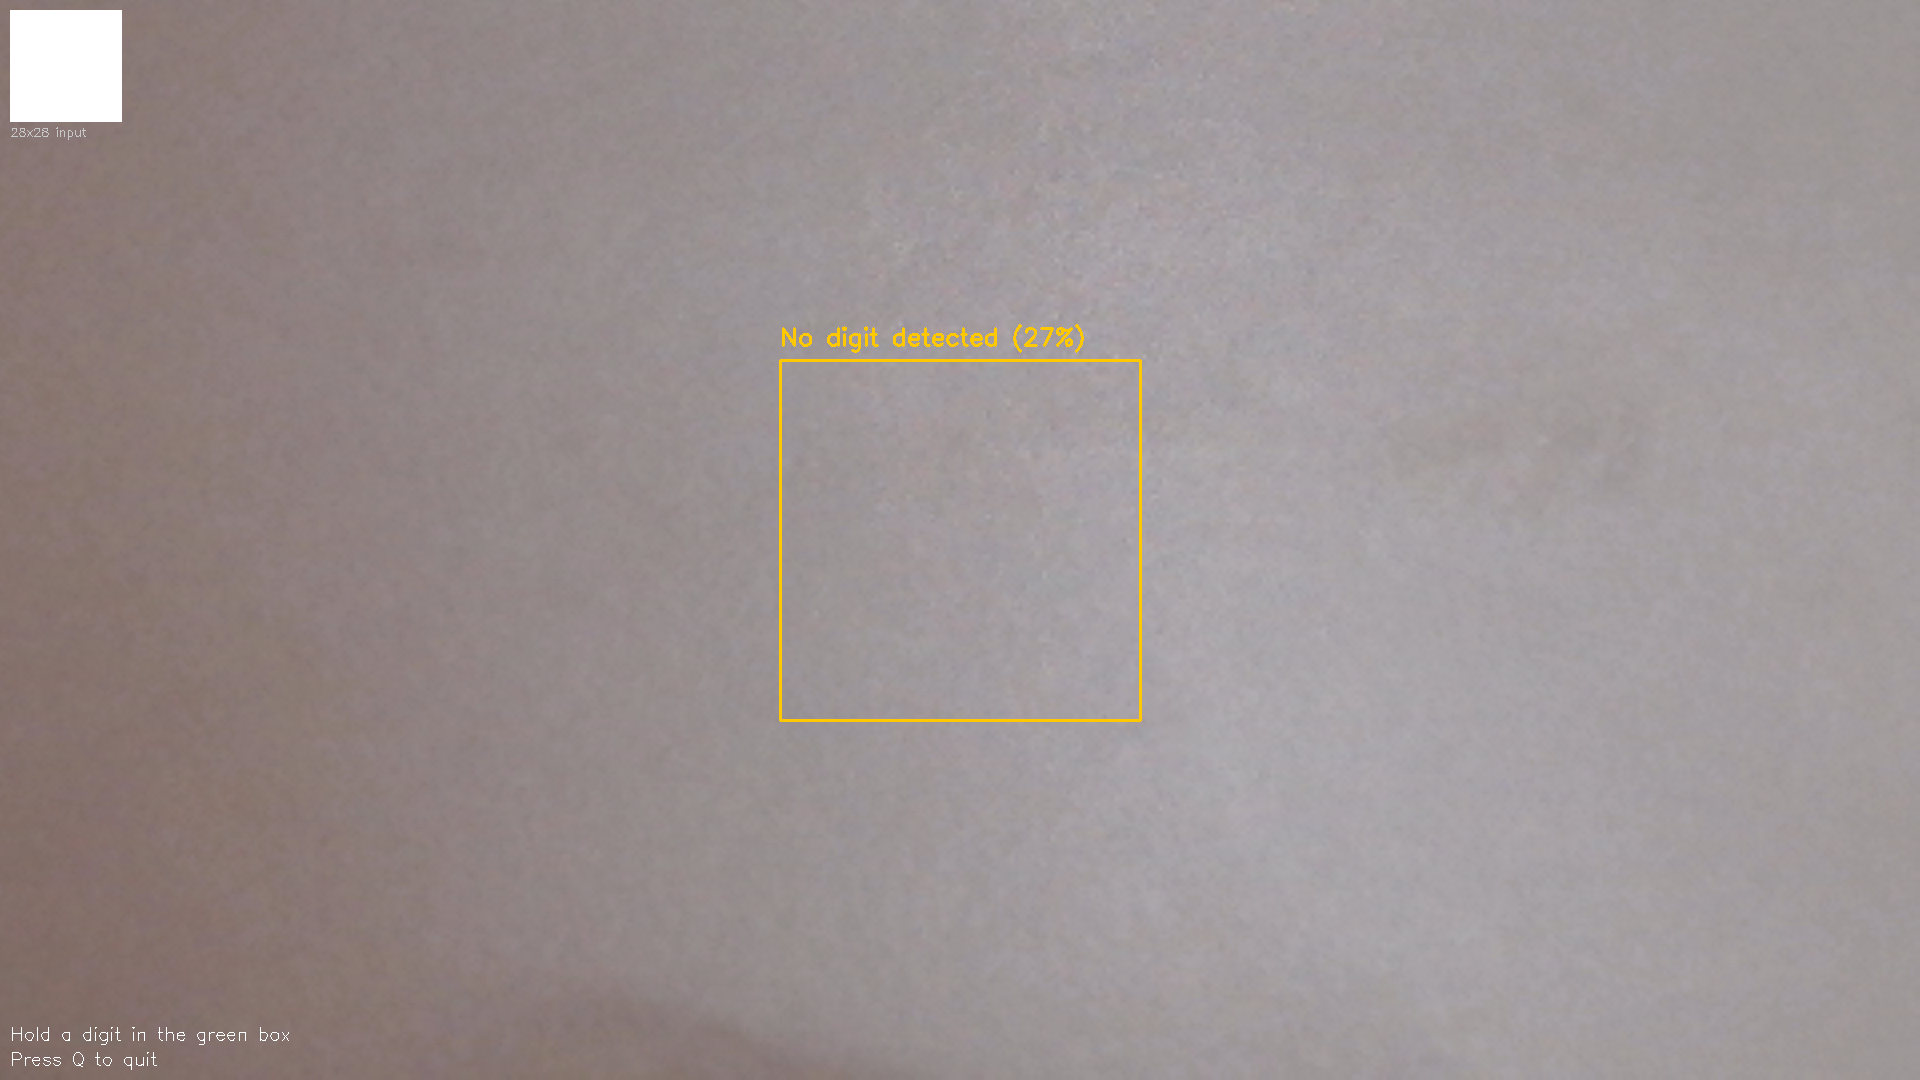
\includegraphics[width=\textwidth]{report_images/live_demo_1.png}
        \caption{No digit detected (blank background)}
    \end{subfigure}
    \hfill
    \begin{subfigure}[b]{0.32\textwidth}
        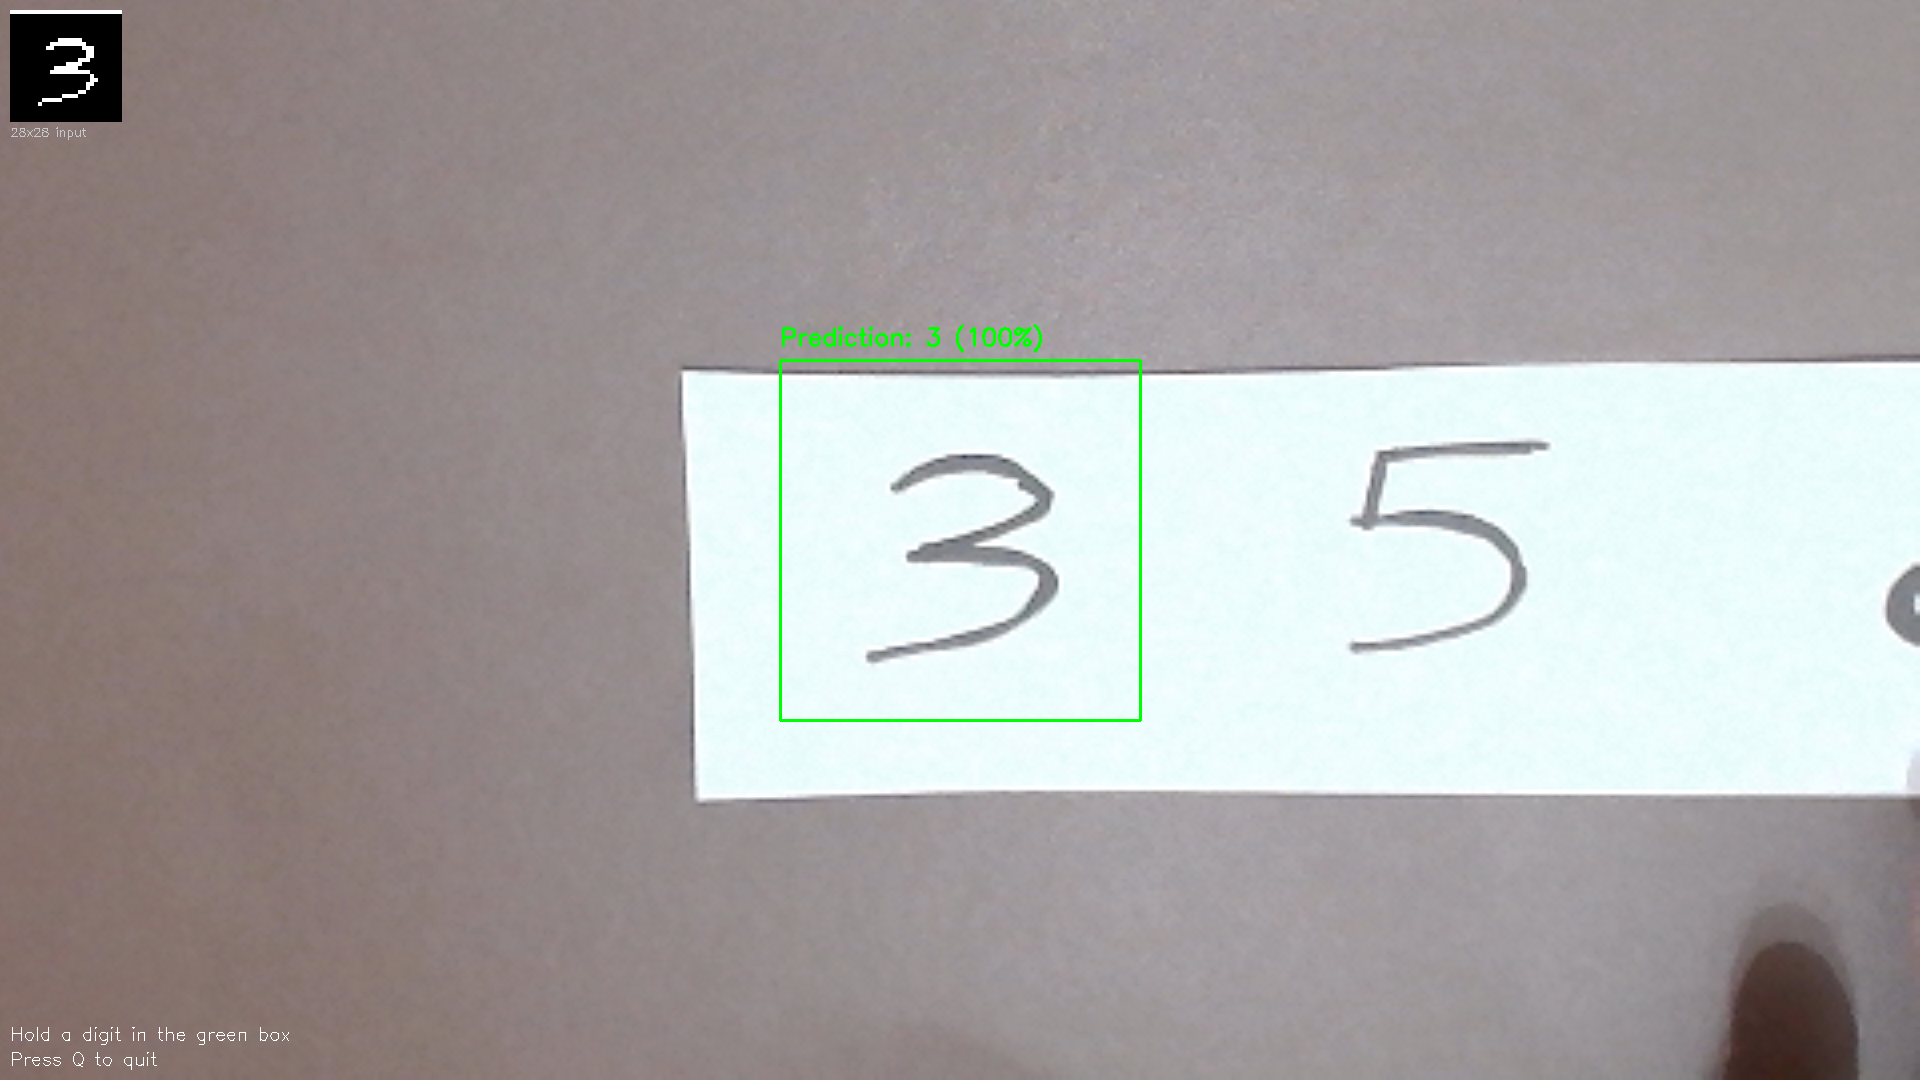
\includegraphics[width=\textwidth]{report_images/live_demo_2.png}
        \caption{Recognizing digit 3}
    \end{subfigure}
    \hfill
    \begin{subfigure}[b]{0.32\textwidth}
        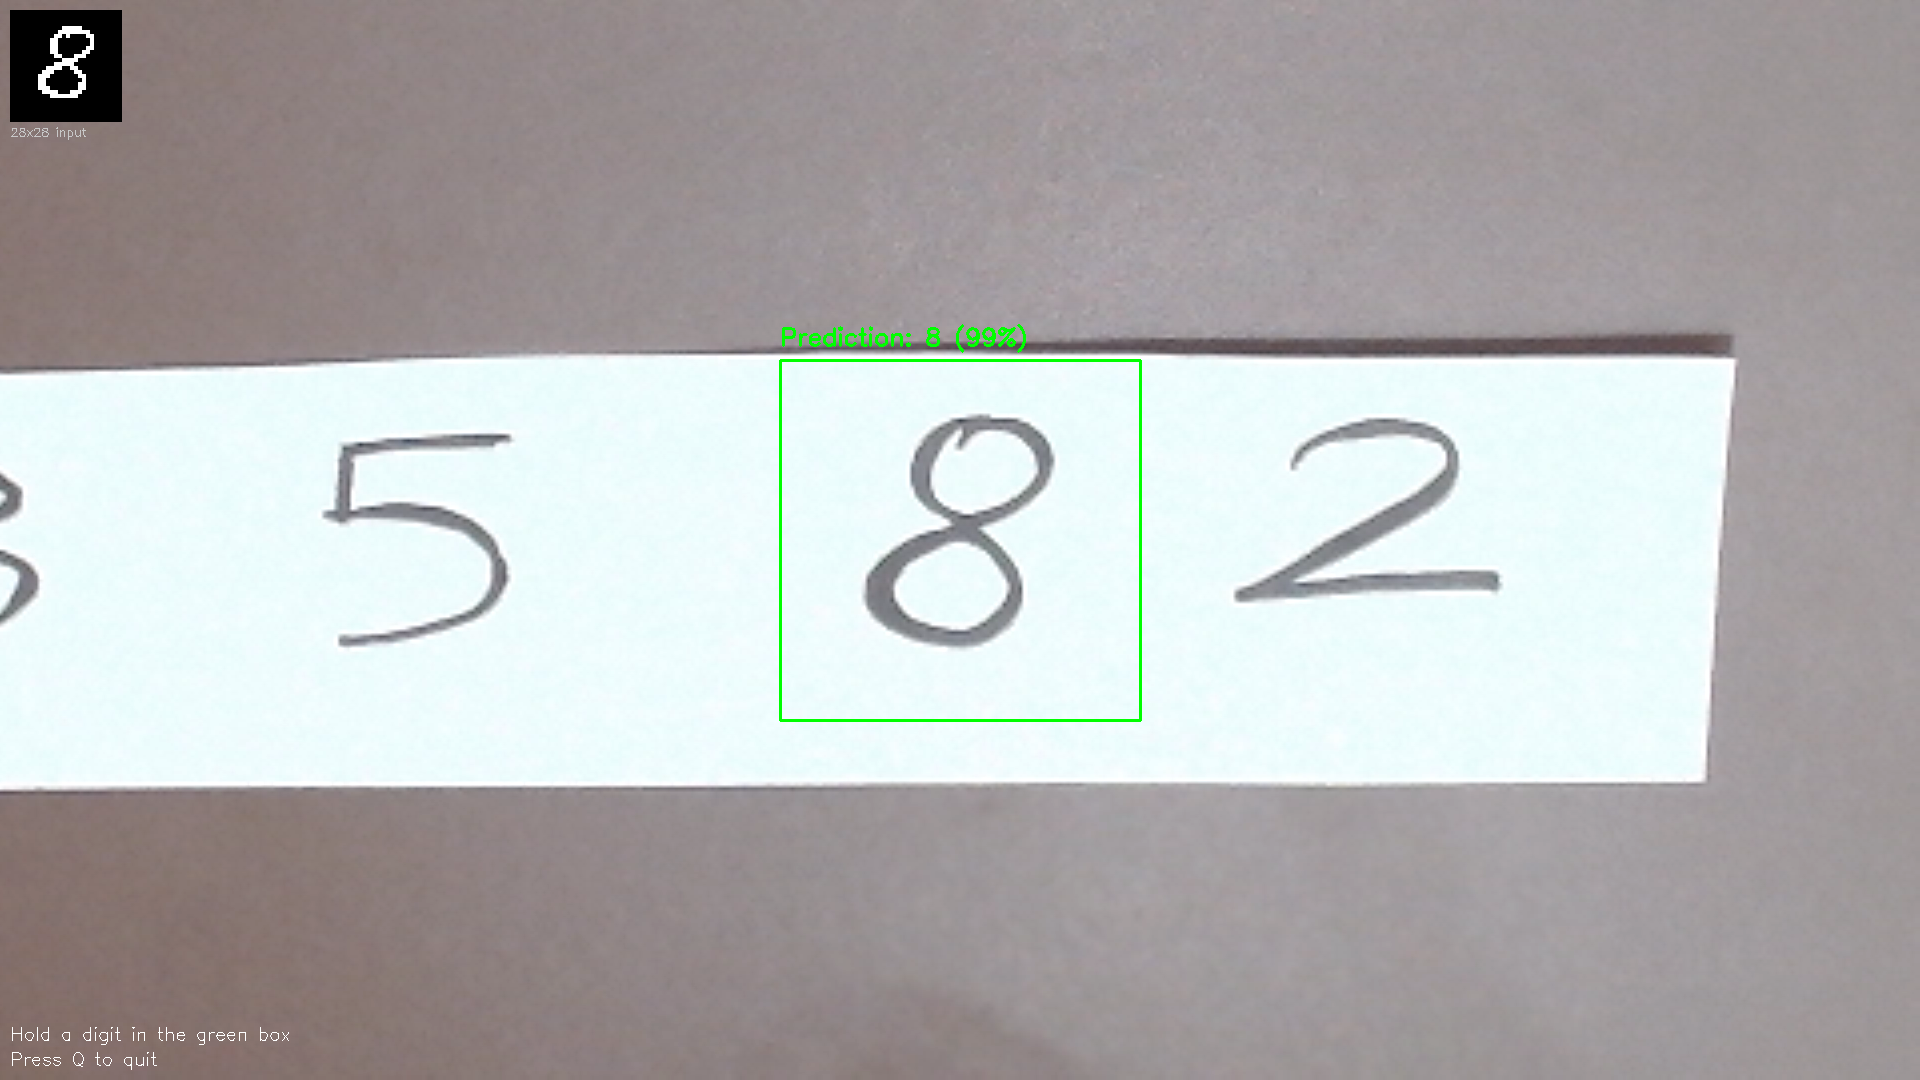
\includegraphics[width=\textwidth]{report_images/live_demo_3.png}
        \caption{Recognizing digit 8}
    \end{subfigure}
    \caption{Live webcam digit recognition. Green box indicates a
    confident prediction, yellow indicates uncertainty. The top-left
    corner shows the preprocessed 28$\times$28 input that the model
    receives.}
\end{figure}

\subsection{Extension 2: Additional Greek Letters}

The transfer learning system was extended from 3 to 6 classes by adding
delta ($\delta$), epsilon ($\varepsilon$), and lambda ($\lambda$).
This required substantial data curation and engineering effort:

\begin{itemize}
    \item \textbf{Custom dataset creation:} 6--11 training images per
    class were hand-drawn, photographed, and cropped to
    128$\times$128. The system auto-detects classes from subdirectory
    names, requiring no code changes to scale.

    \item \textbf{Domain shift diagnosis:} Initial accuracy was
    $\sim$40\%. A systematic diagnostic (isolating 3-class base case)
    proved the root cause was train/test style mismatch, not model
    capacity. See Section~4 for the full iteration log.

    \item \textbf{Morphological preprocessing:} Provided training
    images (thin pencil strokes) were thickened with PIL
    \texttt{MinFilter(5)} to reduce the domain gap with user-drawn
    test images (thick marker).

    \item \textbf{Systematic hyperparameter tuning:} A dedicated
    tuning script (\texttt{greek\_tuner.py}) tested 10 configurations
    across 3 freeze levels, 2 optimizers, and multiple learning rates
    to identify the best transfer learning strategy.
\end{itemize}

These combined efforts raised accuracy from $\sim$40\% to 88\%
on 6 classes with only $\sim$60 total images. An additional challenge
was discovered when images rotated in macOS Finder appeared upright
visually but retained their original pixel orientation via XMP metadata
tags---PIL and PyTorch read the raw pixels, ignoring the tag. A script
was written to apply the rotation to the actual pixel data, which
further improved accuracy from $\sim$79\% to 88\%.

\subsection{Extension 3: Gabor Filter Bank}

Hand-crafted Gabor filters (5 orientations $\times$ 2 frequencies =
10 filters, 5$\times$5) were used as a frozen conv1 replacement. All
other layers (conv2, fc1, fc2) were trained normally for 5 epochs.

\begin{figure}[H]
    \centering
    \begin{subfigure}[b]{0.48\textwidth}
        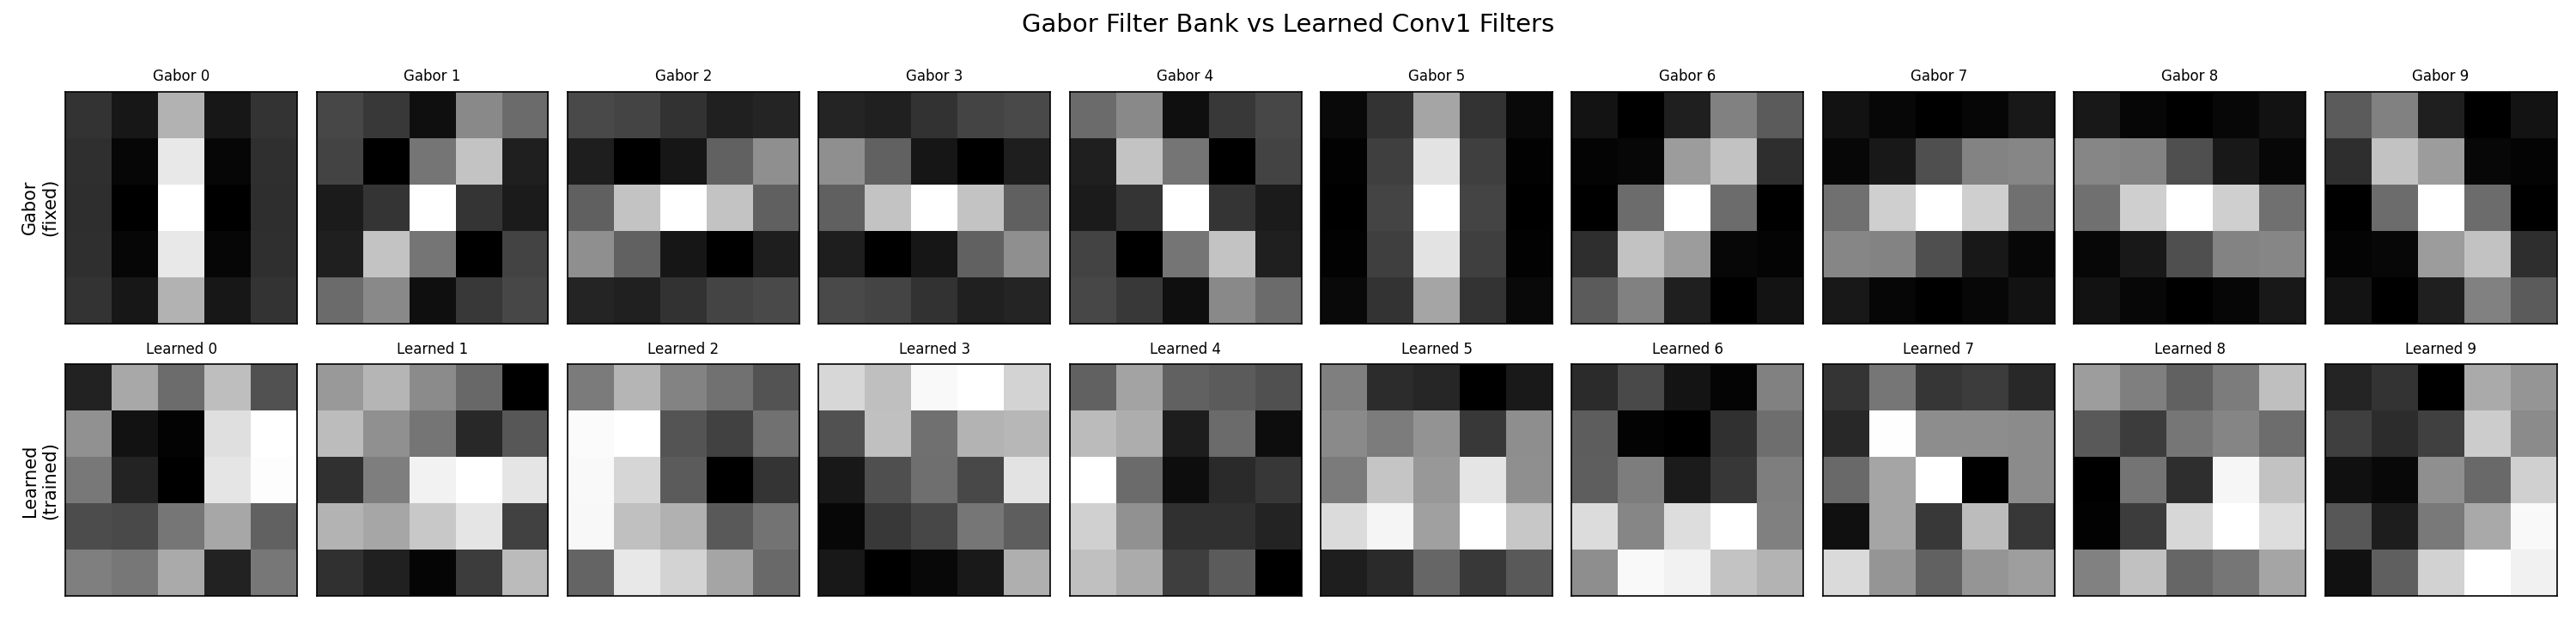
\includegraphics[width=\textwidth]{report_images/gabor_vs_learned_filters.png}
        \caption{Gabor filters vs learned conv1 filters}
    \end{subfigure}
    \hfill
    \begin{subfigure}[b]{0.48\textwidth}
        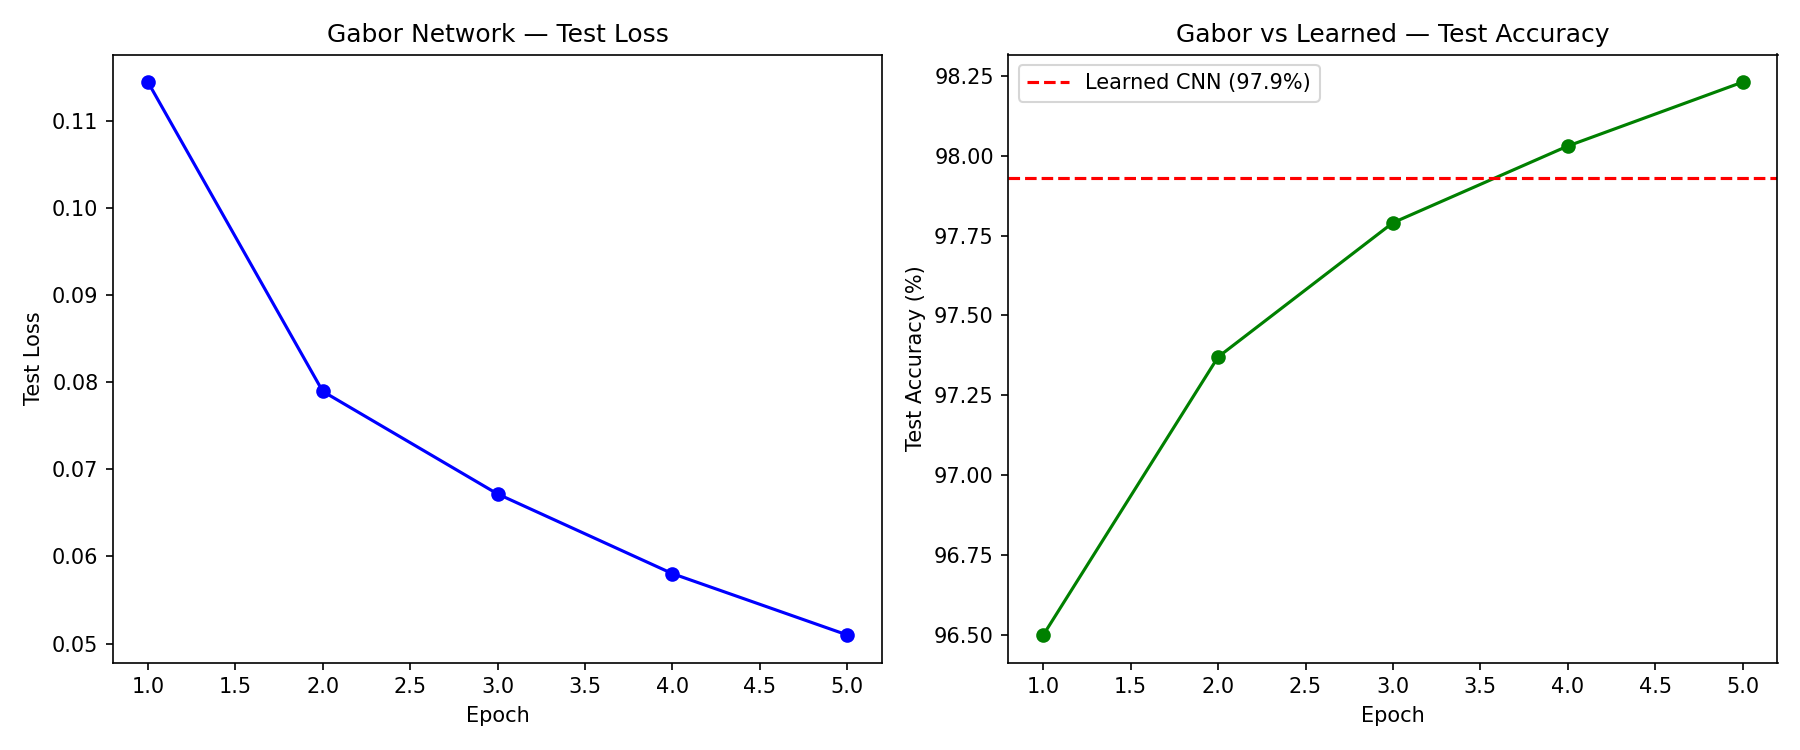
\includegraphics[width=\textwidth]{report_images/gabor_training_results.png}
        \caption{Training accuracy comparison}
    \end{subfigure}
    \caption{Gabor filter bank experiment. The hand-crafted Gabor filters
    (98.23\%) slightly outperform the fully-learned CNN (97.93\%).}
\end{figure}

The Gabor network slightly outperformed the fully-learned CNN,
suggesting that for MNIST, hand-crafted edge detectors at the first
layer are competitive with learned filters. The Gabor filters provide
a strong prior (oriented edges at multiple frequencies) well-suited to
digit stroke patterns, allowing the remaining layers to focus on
higher-level feature combination.

\subsection{Extension 4: Confusion Matrix Analysis}
\label{sec:confusion}

A confusion matrix (\texttt{confusion\_tsne.py}) was generated from
the CNN's predictions on all 10{,}000 MNIST test images
(Figure~\ref{fig:confusion}). The most common misclassification was
2$\to$7 (13 instances), followed by 9$\to$4, 9$\to$1, and 5$\to$3
(10 each). These errors are intuitive: 2 and 7 share a horizontal
stroke and diagonal, while 9 and 4 share a vertical stroke with a
closed or partial loop. Errors are well-distributed across classes
rather than concentrated on any single class, indicating the CNN has
no systematic blind spot.

\begin{figure}[H]
    \centering
    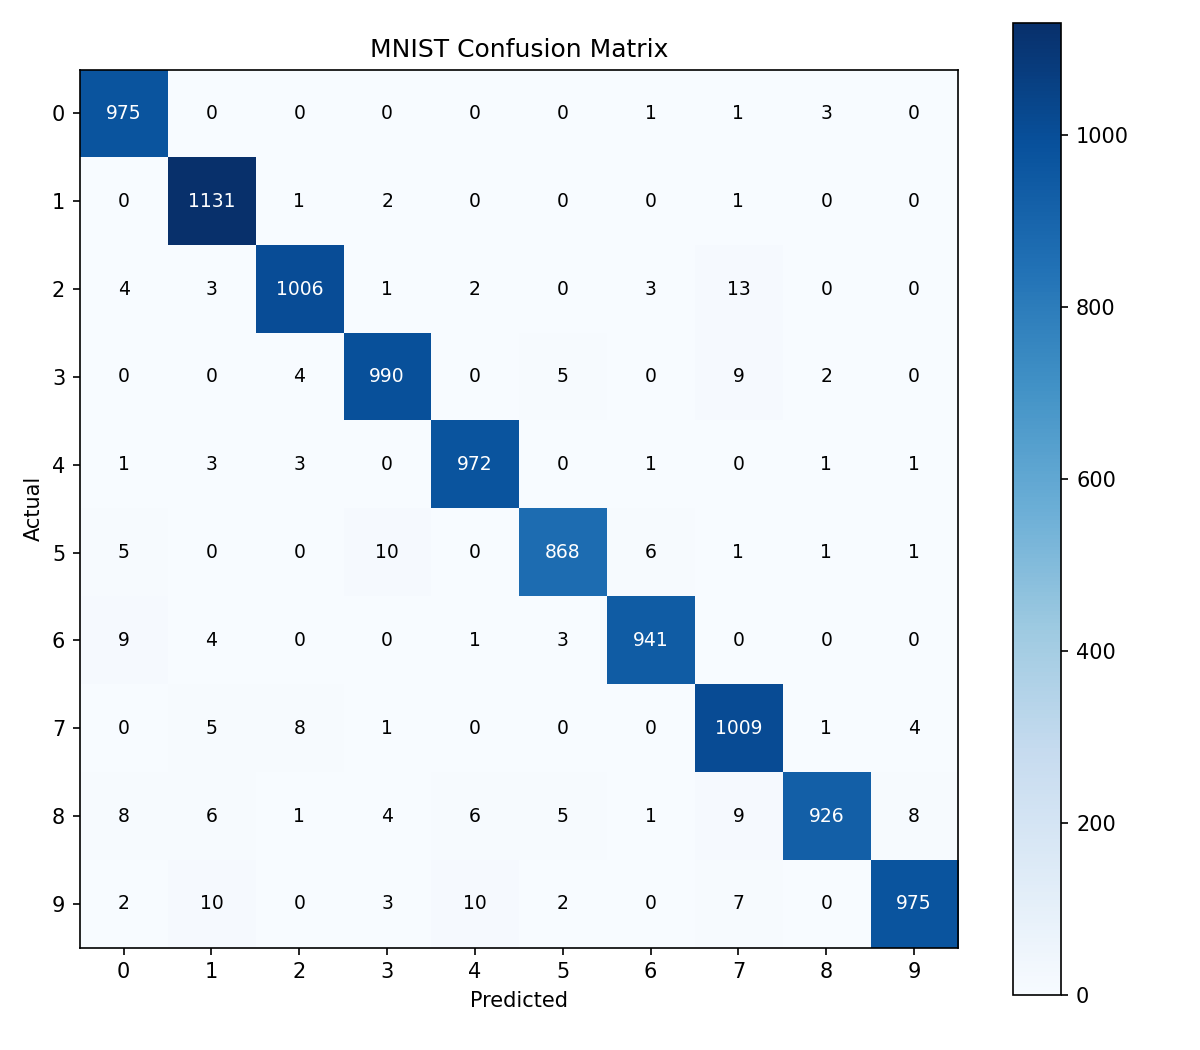
\includegraphics[width=0.6\textwidth]{report_images/confusion_matrix.png}
    \caption{Confusion matrix for the CNN on the MNIST test set. Diagonal
    entries show correct predictions; off-diagonal entries show
    misclassifications. Most errors involve visually similar digit pairs.}
    \label{fig:confusion}
\end{figure}

\subsection{Extension 5: t-SNE Embedding Visualization}

To visualize how the CNN internally represents digits, the
50-dimensional fc1 hidden layer activations were extracted for all
10{,}000 test images and projected to 2D using t-SNE (perplexity=30).
Figure~\ref{fig:tsne} shows that the network learns well-separated
clusters for each digit class, confirming that the penultimate layer
has learned highly discriminative features. Notably, digits that the
confusion matrix (Extension~4) identified as easily confused (e.g.,
4 and 9, 3 and 5) have clusters that are spatially closer in the
embedding, demonstrating that the network's internal representation
directly reflects visual similarity between digit shapes.

\begin{figure}[H]
    \centering
    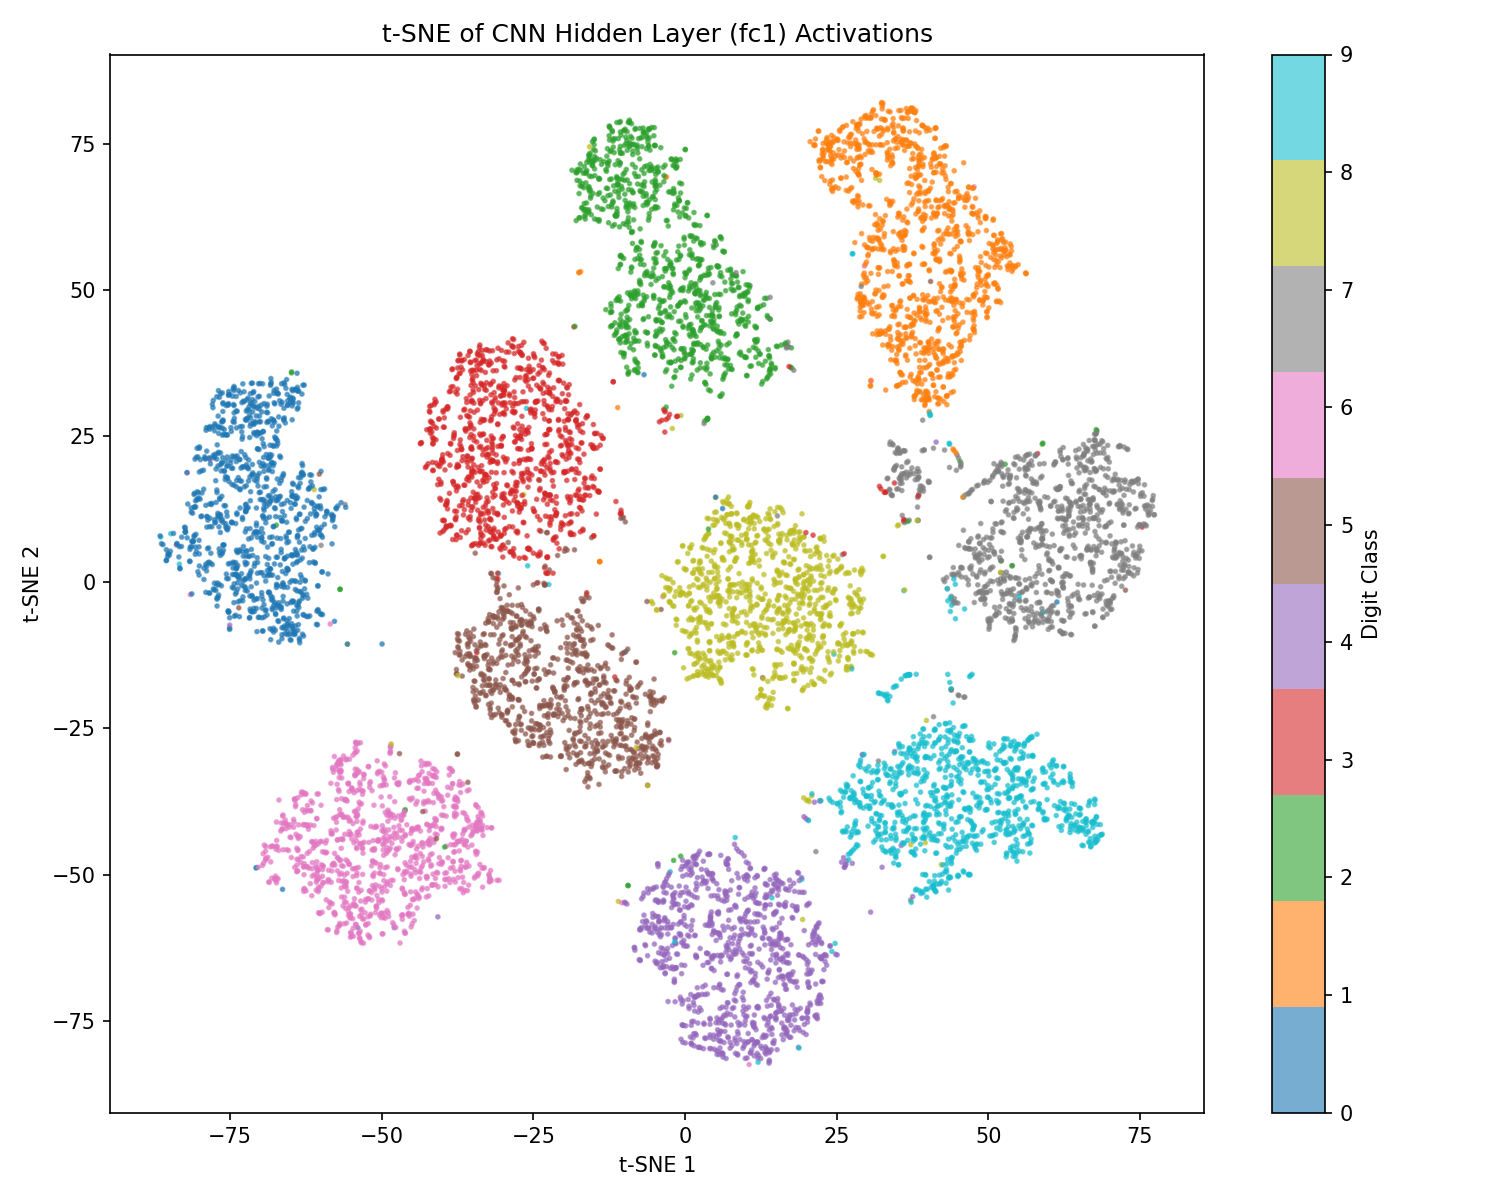
\includegraphics[width=0.7\textwidth]{report_images/tsne_embedding.png}
    \caption{t-SNE projection of fc1 hidden layer activations. Each point
    is one test image, colored by digit class. The clean separation shows
    the CNN has learned discriminative features, while nearby clusters
    (e.g., 4/9, 3/5) correspond to visually similar digits.}
    \label{fig:tsne}
\end{figure}

\subsection{Extension 6: Data Augmentation Experiment}

An augmentation experiment (\texttt{augmentation\_experiment.py}) trained
two identical CNN architectures for 5 epochs: one with the standard
MNIST pipeline (baseline) and one with random rotation ($\pm 15^\circ$)
and random affine translation (up to 10\% shift). Both models were
evaluated on the unaugmented test set.

\begin{figure}[H]
    \centering
    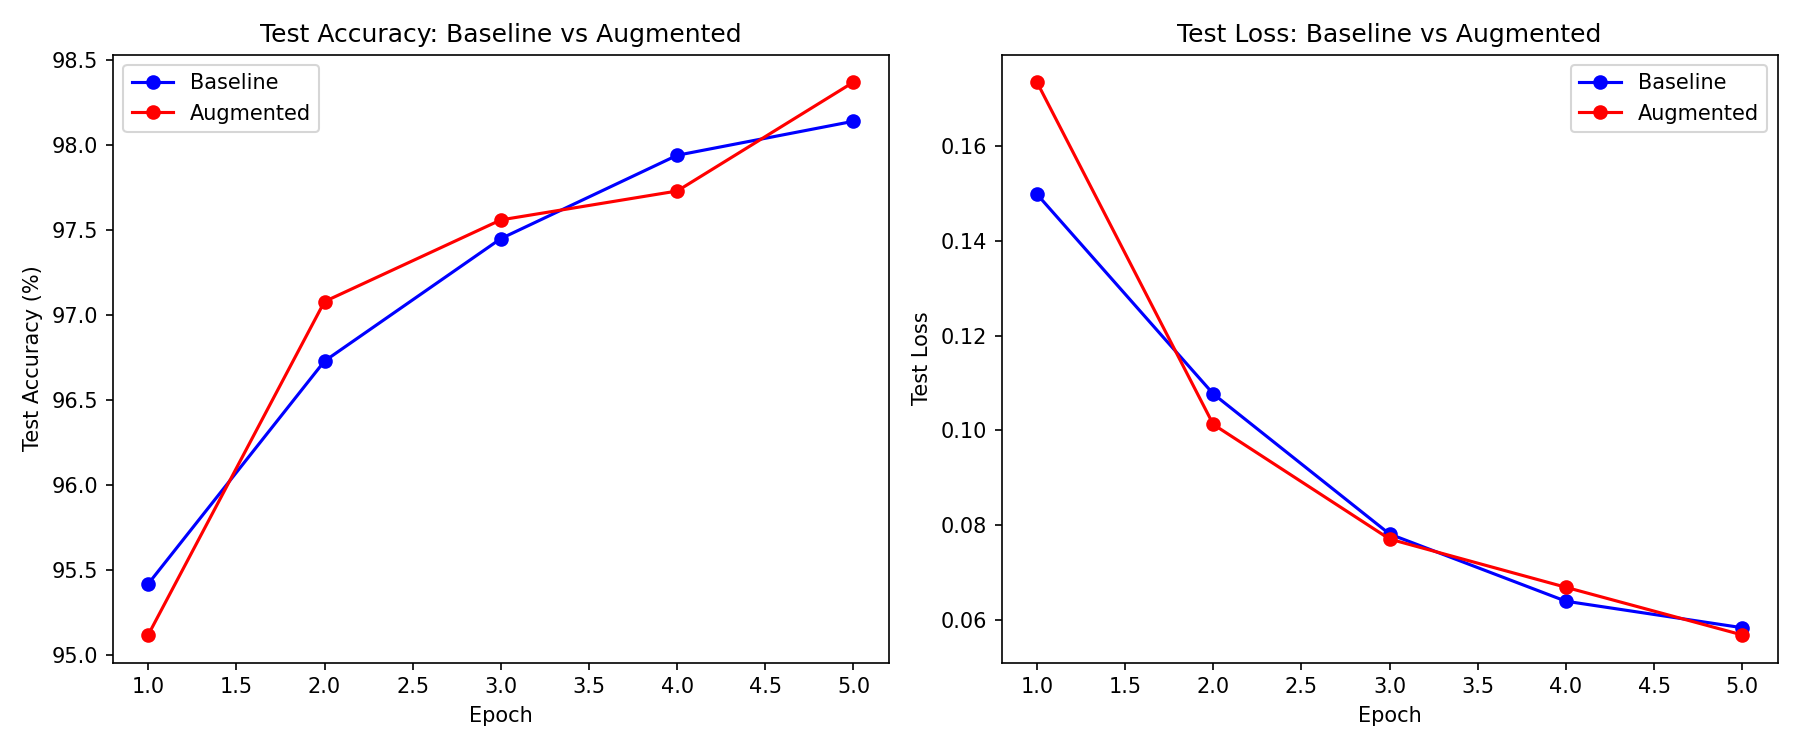
\includegraphics[width=0.8\textwidth]{report_images/augmentation_comparison.png}
    \caption{Test accuracy and loss for baseline vs augmented training.
    Augmentation reduces overfitting (lower train accuracy) while slightly
    improving generalization.}
    \label{fig:augmentation}
\end{figure}

The augmented model achieved 98.37\% test accuracy versus 98.14\% for the
baseline---a modest 0.23\% improvement. However, the train-test accuracy
gap reveals the real story: the baseline's gap was $-1.58$\% (train
96.56\%, test 98.14\%), while the augmented model's gap was $-7.31$\%
(train 91.06\%, test 98.37\%). The augmented model's much lower training
accuracy reflects the harder augmented training distribution, while its
higher test accuracy confirms better generalization. On MNIST, where the
baseline is already near-saturated, the benefit is small; augmentation
would have a larger impact on harder datasets or smaller training sets.

% ---------------------------------------------------------------
\section{Reflection}
% ---------------------------------------------------------------

The transfer learning task was the most instructive. The severe impact
of training/test domain shift---thin pencil strokes vs thick marker---on
a tiny dataset (60 images) demonstrated that data quality and
distribution matching matter as much as model architecture. Building a
systematic tuning script replaced guesswork with evidence, and the
decisive insight was diagnostic: isolating the 3-class base case proved
the problem was data distribution, not model capacity.

The Fashion MNIST experiment reinforced that architectural choices
interact. Dropout's benefit depended on model size: useless for a small
network trained briefly, but valuable once the network grew. This makes
isolated hyperparameter tuning insufficient---the two-round linear
search captured this interaction efficiently.

The Gabor filter result was the most surprising: classical computer
vision priors competed with learned features on MNIST, suggesting that
domain knowledge remains valuable even in the deep learning era.

% ---------------------------------------------------------------
\section{Acknowledgements}
% ---------------------------------------------------------------

\begin{itemize}
    \item Professor Bruce Maxwell for the assignment guidelines,
    the alpha/beta/gamma Greek letter training images, and the
    \texttt{NetTransformer} class template.
    \item Claude Code (Anthropic) for assistance with code structure
    and commenting conventions, programmatic cropping and centering
    of training/test images to uniform size, data/model evaluation
    visualization code (plotting, confusion matrix, t-SNE), and
    templating the \LaTeX{} report structure.
    \item PyTorch documentation and tutorials.
    \item MNIST dataset (LeCun et al.) and Fashion MNIST dataset
    (Xiao et al.).
\end{itemize}

\end{document}
